

\documentclass[a4paper, 12pt, notitlepage]{report}
\usepackage[T1]{fontenc}
\usepackage{textcomp}
\usepackage{xfrac}
\usepackage{bm}

\usepackage[utf8]{inputenc}
\usepackage[english,italian]{babel}
\usepackage{verbatim}
\usepackage{listings}

\usepackage{hyperref}
\usepackage{etoc}

\usepackage{float}
\usepackage{amsmath}
\usepackage{amsthm}
\usepackage{amsfonts}
\usepackage{mathtools}

\usepackage{fancyvrb}

\usepackage{xargs}
\usepackage[pdftex,dvipsnames,table,xcdraw]{xcolor}

\usepackage{xcolor}

\usepackage{graphicx} % graphics package
\usepackage{subcaption}
\graphicspath{ {./media/} } % images folder path


\usepackage{geometry}
\geometry{
    a4paper,
    top=30mm,
    bottom=30mm,
    left=35mm,
    right=35mm
}

\usepackage[pagestyles]{titlesec}
\titleformat{\chapter}[display]{\normalfont\bfseries}{}{0pt}{\Huge}

\newpagestyle{main}{
    \sethead[\thepage][][\chaptertitle]
        {}{}{\thepage}
    \setfoot[][][]
        {}{}{}
}

\usepackage[section]{placeins} % utilizzare /FloatBarrier alla fine della definizione delle figure per non farle scivolare in altre sezioni o altro

\renewcommand*\contentsname{Index}

% remove new paragraph indentation
\setlength{\parindent}{0cm}

% colors for code snippets
\definecolor{codegreen}{rgb}{0,0.7,0.5}
\definecolor{codegray}{rgb}{0.5,0.5,0.5}
\definecolor{codeblue}{rgb}{0,0.5,0.82}
\definecolor{backcolour}{rgb}{0.95,0.95,0.95}

\lstdefinestyle{main}{
    backgroundcolor=\color{backcolour},
    commentstyle=\color{codegreen},
    keywordstyle=\color{orange},
    numberstyle=\tiny\color{codegray},
    stringstyle=\color{codeblue},
    basicstyle=\ttfamily\footnotesize,
    breakatwhitespace=false,
    breaklines=true,
    captionpos=b,
    keepspaces=true,
    numbers=left,
    numbersep=5pt,
    showspaces=false,
    showstringspaces=false,
    showtabs=false,
    tabsize=2
}
\lstset{style=main}

\newtheoremstyle{thmstyle}
	{\topsep}% measure of space to leave above the theorem. E.g.: 3pt
	{\topsep}% measure of space to leave below the theorem. E.g.: 3pt
	{}% name of font to use in the body of the theorem
	{}% measure of space to indent
	{\bfseries}% name of head font
	{ }% punctuation between head and body
	{.1em}% space after theorem head; " " = normal interword space
	{\thmname{#1}}% Manually specify head
\theoremstyle{thmstyle}

\newtheorem{example}{Example}



% front page created with \title command
\title{
    
\includegraphics[scale=0.2]{unilogo.png}
    
    \vspace{1cm}{
        \large{\textbf{UNIVERSIT\`{A} DEL SALENTO}}
    }
        
    \normalfont{Relazione di Laboratorio}
    \par\noindent\rule{\textwidth}{0.4pt}
    
    \vspace{0.3cm}
    \small{Mirko Caforio, Alessandro Convertino, Raffaele Crusi, Federico Izzi, Giovanni Pepe, Matteo Rosato, Antonio Scelsi, Ludovico Scurti}
    
    \vspace{1.0cm}
    \large{??????}

    
    \vspace{4.0cm}
    
    \par\noindent\rule{\textwidth}{0.4pt}
    \vspace{0.3cm}
    
    \small{ACADEMIC YEAR 2022/2023}
    \thispagestyle{empty}
}

\author{}
\date{}

\hypersetup{hidelinks}


\begin{document}
    % front page creation
    \maketitle
    \thispagestyle{empty}

    % blank page
    \newpage
    \mbox{}
    \thispagestyle{empty}
    
    % index creation
    \hypersetup{hidelinks}
    \tableofcontents
    \addtocontents{toc}{\protect\thispagestyle{empty}}
    \thispagestyle{empty}

    % Chapter: "Introduction"
    \hypersetup{hidelinks}
    \chapter{Introduzione}
\label{chap:introduction}
\section{antoniogay}
\label{sect:gay}
TEST.


    % Chapter 2
    \hypersetup{hidelinks}
    

\chapter{Misure di Resistenza ed Impedenza con DMM e LCR}
\label{chap:prima_prova}


\section{obbiettivi}
\label{sec:ob1}


L'obiettivo primario di questa iniziale esperienza di laboratorio consiste nell'acquisire familiarità con l'utilizzo di strumentazione di base per le misurazioni, con le corrette procedure di misurazione e con la valutazione dell'incertezza associata, nel caso di misurazioni di resistenza e impedenza.
\newline \newline
A tale scopo ci è stato dato un resistore dal valore nominale di 1,5 $\Omega$ (valore nominale apprezzabile ad occhio nudo, tramite la visualizzazione delle lineette di colore marrone, verde, oro (vedi figura \ref{fig:resistore})) con un incertezza del 5\% (dato che l'ultimo anello è di colore oro).

\begin{figure}[h]
    \centering
    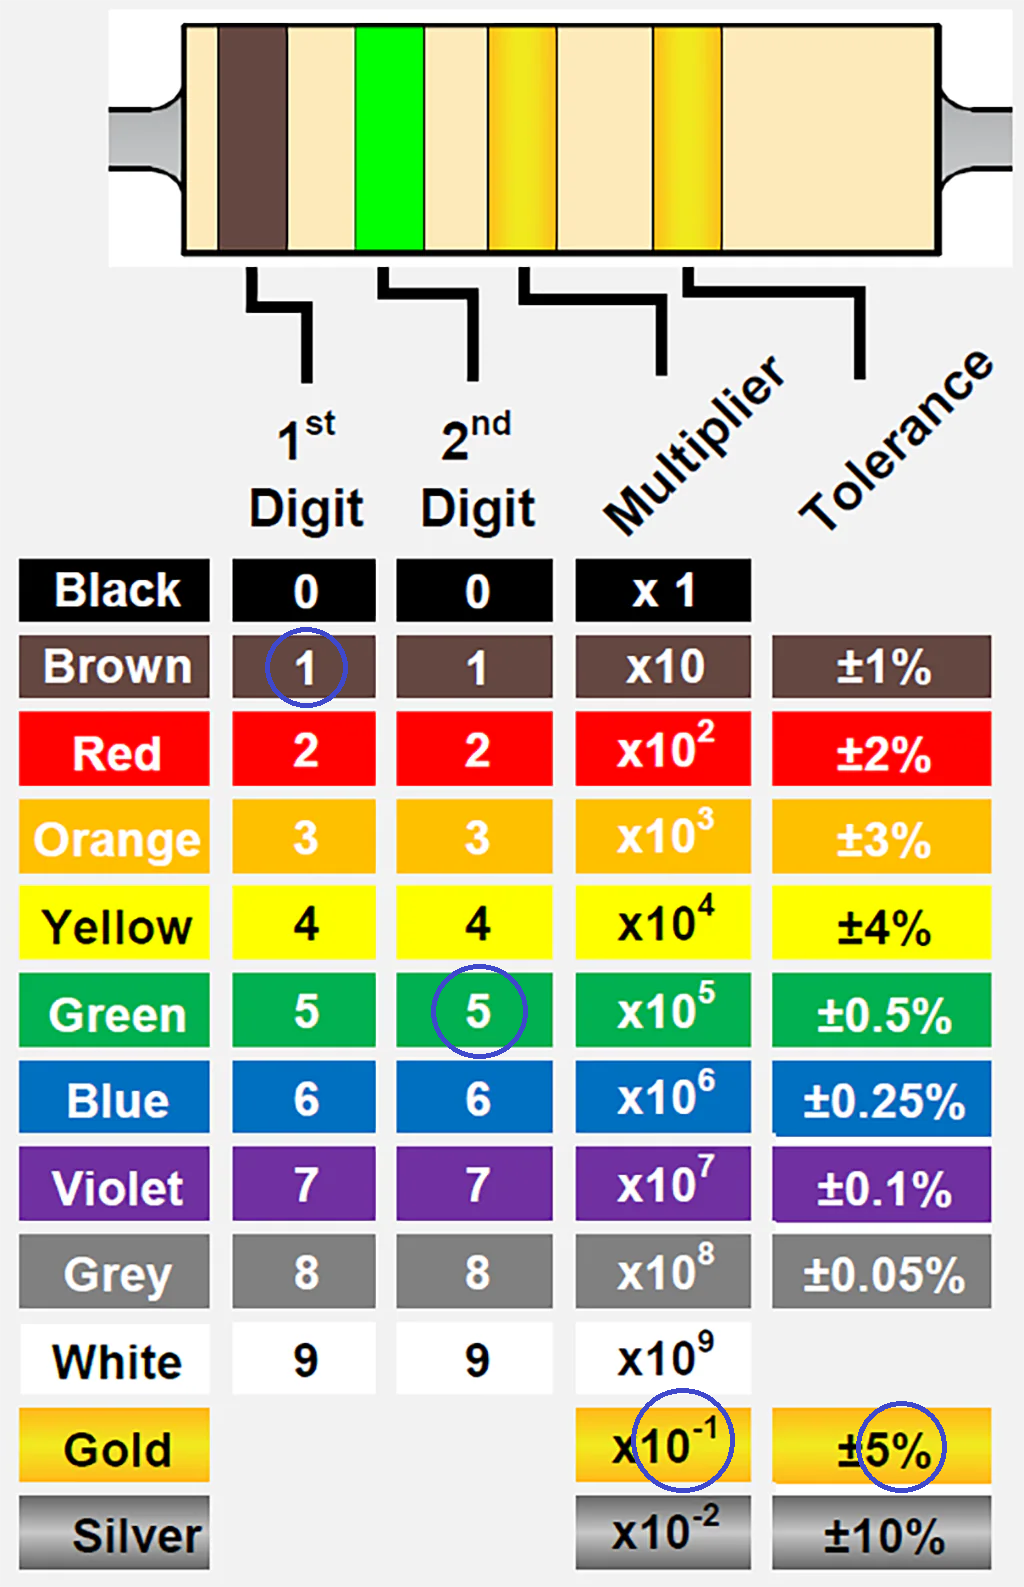
\includegraphics[height=10cm]{Relazione/media/resistoretab.png}
    \caption{Tabella che raffigura il codice dei colori di un resistore}
    \label{fig:resistore}
\end{figure}















\section{Misure di resistenze con multimetro portatile}
\label{sec:mult_port}

\begin{figure}[h]
    \centering
    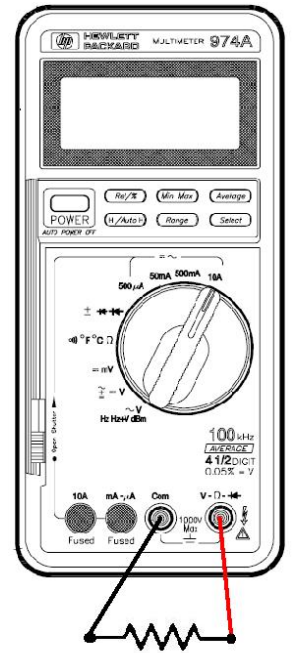
\includegraphics[height=10cm]{Relazione/media/multimetro_port.png}
    \caption{Multimetro utilizzato (Hewlett Packard 974A)}
    \label{fig:multimetro_port}
\end{figure}

Il multimetro HP 974A è dotato di un display a 4 ½ cifre, il quale rappresenta uno strumento con 4 cifre principali e un'ulteriore cifra riservata per indicare il segno e, eventualmente, il valore della cifra più significativa della misurazione. Per calcolare la resistenza con un valore nominale dichiarato dal produttore pari a (1500 ± 7,5) m$\Omega$, abbiamo utilizzato il pulsante "RANGE" per impostare il valore di fondo scala, ovvero il limite superiore che il multimetro può "misurare", a 500 $\Omega$. Dato che lo strumento ha un campo di misura pari a 1/50000 del valore di fondo scala, il passo di quantizzazione, indicato come "Q", è pari a
\begin{equation}
    Q = \frac{V_F_S}{50000} = \frac{500}{50000} = 10 m\Omega
\end{equation}
con un incertezza di quantizzazione pari a: 
\begin{equation}
    U_q = \frac{Q}{2} = 5 m\Omega
\end{equation}

Procediamo con la valutazione dell'incertezza di \textbf{tipo B}, basata sull'utilizzo di informazioni note a priori quali le specifiche metrologiche degli strumenti adoperati. L’incertezza del dispositivo è data da una formula binomia composta da una parte proporzionale alla lettura e da un’altra pari a un numero fisso di LSB, quindi 
 proporzionale alla portata. Le specifiche del costruttore dello strumento, per misure di resistenze, sono le seguenti:

\begin{figure} [h]
    \centering
    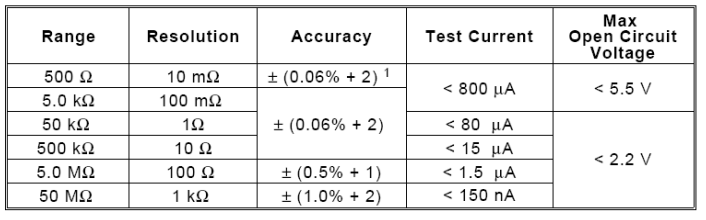
\includegraphics[height=5cm]{Relazione/media/incertezza_port.png}
    \caption{Specifice di incertezza dello strumento utilizzato (Hewlett Packard 974A)}
    \label{fig:Incertezza_multimetro_port}
\end{figure}

Avendo impostato un valore di fondo scala pari a 500 $\Omega$ possiamo notare dalla precedente tabella un’incertezza pari a ±(0,06\% + 2) $\Omega$ , dove il primo termine è proporzionale alla lettura e il secondo alla portata. Si noti che per misure di ampiezza è possibile definire un modello semplificato di uno strumento per misure statiche, del tipo:

\begin{figure} [h]
    \centering
    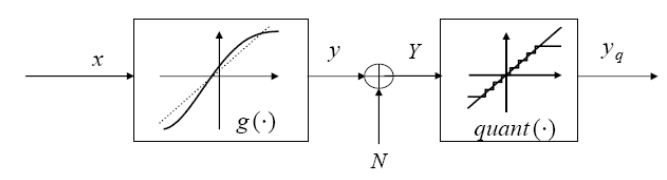
\includegraphics[height=3cm]{Relazione/media/modello_semplificato.png}
    \label{fig:modello}
\end{figure}

Su cui definiamo un errore totale sulla misura del tipo:

\begin{figure} [h]
    \centering
    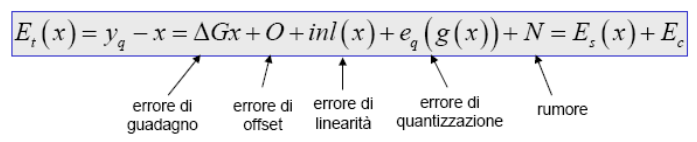
\includegraphics[height=2cm]{Relazione/media/errore_port.png}
    \label{fig:errore port}
\end{figure}

Attraverso una serie di passaggi otteniamo l'incertezza come:
\begin{equation}
    |E_t| \equiv |y_q - x| \equiv | \Delta G_x + O + inl(x) + e_q(g(x)) | \leq 
\end{equation}
(applichiamo una disuguaglianza triangolare)
\begin{equation}
    \leq | \Delta G_x | + | O | + | inl(x) | + | e_q(g(x)) | \leq 
\end{equation}
(applichiamo una disuguaglianza errore-incertezza)
\begin{equation}
    \leq U_G|x| + U_o + U_i_n_l + U_q \cong U_G|y_q| + U_o + U_i_n_l +U_q \equiv U_t_o_t
\end{equation}

Dove, ipotizzando di unire l'incertezza di non linearità integrale nell'incertezza di portata, posso scrivere $U_g$ (incertezza di guadagno), $U_o$ (incertezza di portata dell'offset) e $U_q$ (incertezza di quantizzazione) come: 
\begin{equation}
    \left\{ \begin{array}{rcl}
| \Delta G_x \cdot y_q | \leq U_G |y_q|,    con U_g=0,06\%
\\ | O + inl(x) + e_q(g(x)) | \leq U_o_+_i_n_l_+_q, con U_o_+_i_n_l_+_q=2LSB
\end{array}\right
\end{equation}
Quindi, chiamando Q, passo di quantizzazione e $V_L$ valore letto (supponiamo di usare il primo valore letto nella tabella \label{mult_port}):
\begin{equation}
    U(R) \equiv U_G \cdot V_L + U_o_+_i_n_l_+_q \cdot Q \equiv 0,06\% \cdot 1,62\Omega + 2 \cdot 0,01 \Omega \equiv (0,972 + 20) m\Omega \equiv 0,03 \Omega
\end{equation}
,sapendo che possiamo esprimere la resistenza misurata $R_M$ e il range della resistenza r(R) come:
\begin{equation}
    R_M \equiv(1,62 \pm 0,03) \Omega
\end{equation}
\begin{equation}
    r(R) \equiv [1,59 \Omega \div 1,65 \Omega]
\end{equation}
V\'a notato che l'inclusione dell'errore di non linearit\'a integrale nel secondo termine dell'incertezza fornita dal produttore ( proporzionale alla portata) rende tale termine non solamente un errore di offset puro, ma include anche l'errore di quantizzazione. Pertanto, nel caso di differenze tra misurazioni, non possiamo semplicemente sottrarre l'errore di offset.
Notiamo, usando la resistenza nominale di $(1500 \pm 7,5) m\Omega$ e graficandola con la (2.9) che i due range di valori non sono compatibili.

\begin{figure}[h]
    \centering
    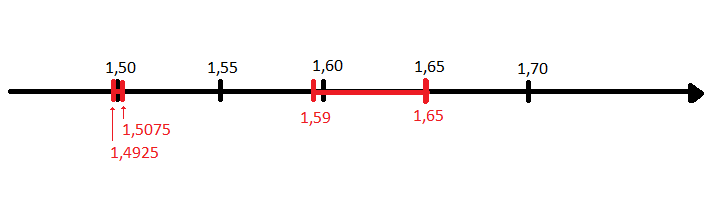
\includegraphics[height=2cm]{Relazione/media/range.png}
    \caption{Differenza dei due range}
    \label{fig:range}
\end{figure}

Effettivamente, la misura eseguita utilizzando il multimetro portatile fornisce una stima non corretta poiché include errori casuali a causa della singola misurazione anziché una media di più valori letti. Inoltre, lo strumento non consente la compensazione degli errori sistematici poiché non dispone di funzioni di calibrazione. Infine, non si è tenuto conto degli errori dovuti alle resistenze di contatto tra i cavi, i puntali e il resistore. Il contributo di tutti questi effetti influisce sul risultato finale della misura.

Se vogliamo quantificare l'accuratezza della misura, assumiamo come valore "vero" della grandezza misurata il valore nominale della resistenza. Facendo questa assunzione, possiamo ottenere una stima dell'errore sistematico come differenza tra il risultato della misura e il valore nominale del componente misurato:
\begin{equation}
    E_S \equiv 1,62 - 1,50 = 0,12\Omega
\end{equation}
L’accuratezza relativa “a” di una misura può essere espressa in funzione di tale errore 
stimato in errore relativo mediante la seguente espressione: 
\begin{equation}
    a \equiv 1 - | \frac{E_S}{R_N_O_M_I_N_A_L_E} | \equiv 92\%
\end{equation}

\newline \newline
\boldsymbol{La} \boldsymbol{nostra} \boldsymbol{prova} \newline

\begin{figure}[h]
    \centering
    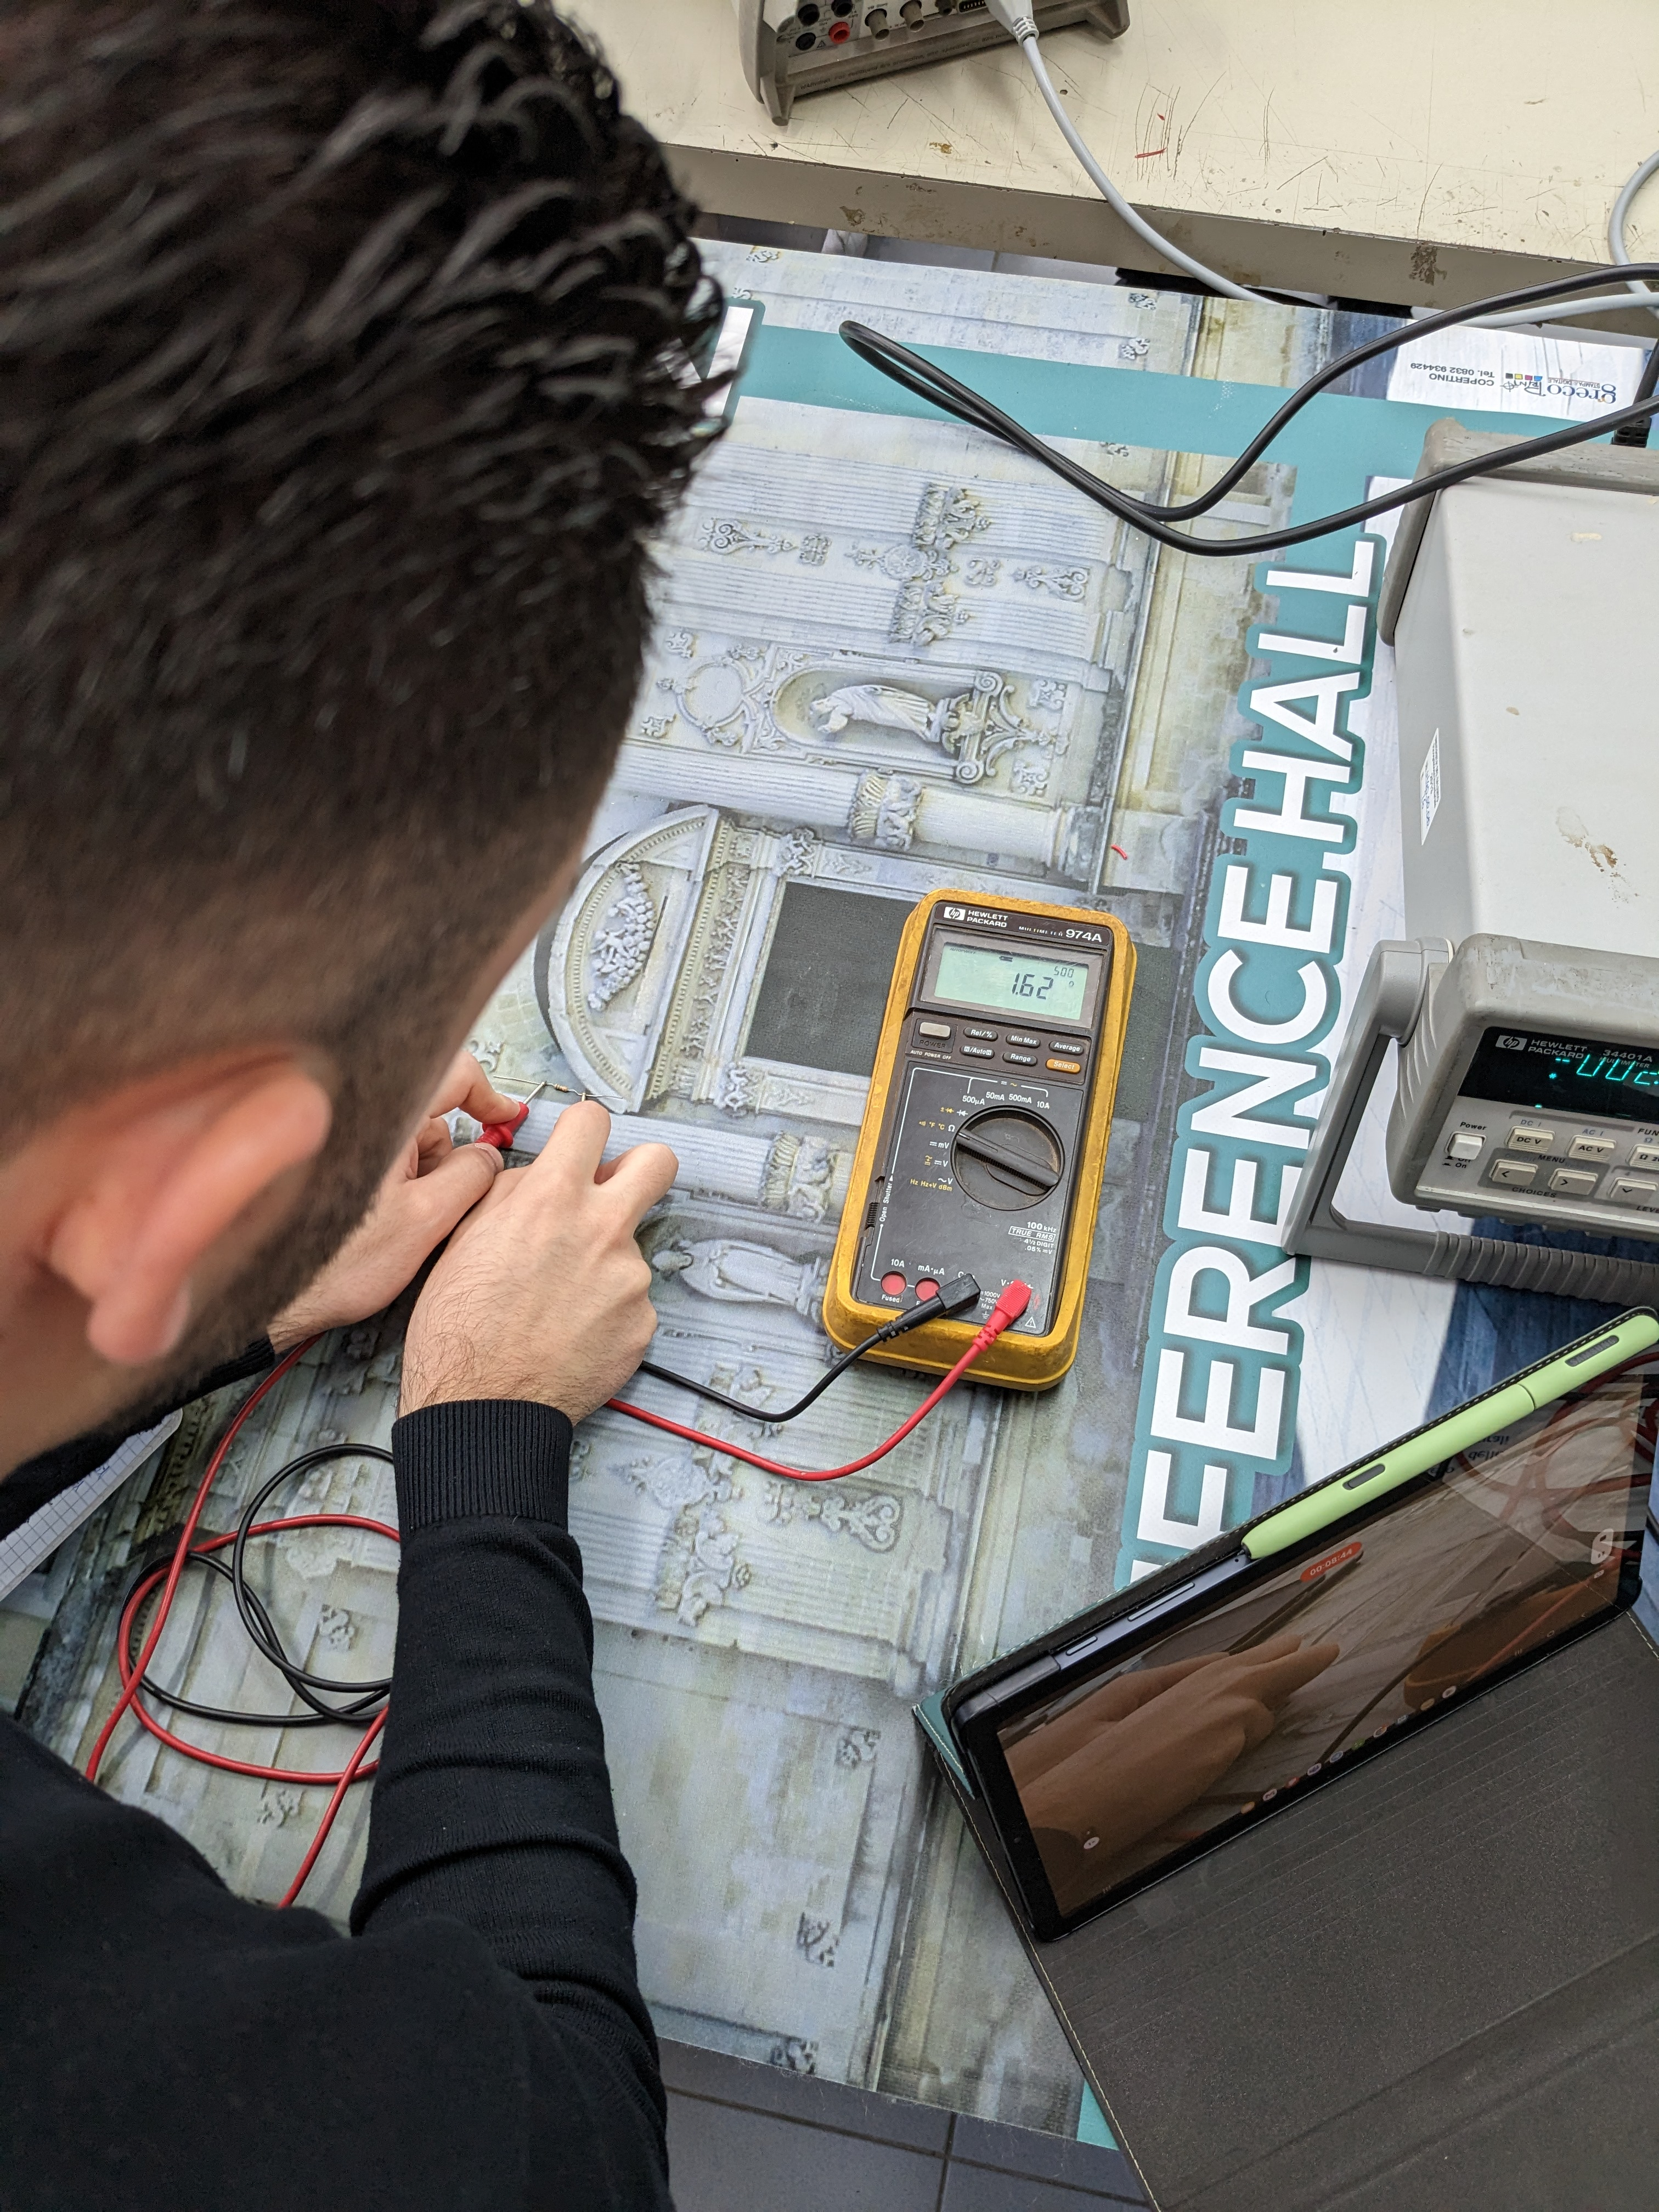
\includegraphics[height=6cm]{Relazione/media/Gameboy_62.jpg}
    \label{fig:mult_port_nostro}
\end{figure}

Quando usiamo il multimetro portatile abbiamo disposto i puntali in maniera pi\'u stabile possibile, applicando una buona pressione per ottenere una misurazione pi\'u fedele possibile,
Abbiamo fatto 10 ripetizioni in modo da ricavare l'incertezza totale, con il contributo valutato di tipo B relativamente alla specifica di strumento utilizzato.

%Per chi vuole inserire tabella usare: https://www.tablesgenerator.com/latex_tables#
%Basta fare ctrl+v sulla tabella di google sheets e andare sul sito , premere File, e fare "Paste table data"

\begin{table}[h]
\centering
\begin{tabular}{|c|c|c|c|}
\hline
\rowcolor[HTML]{6FA8DC} 
Fondo scala 500$\Omega$ & Passo Q ($\Omega$) & Incertezza Uq ($\Omega$) & Incertezza \\ \hline
1,62             & 1,00E-02    & 5,00E-03          & 2,10E-02   \\ \hline
1,61             & 1,00E-02    & 5,00E-03          & 2,10E-02   \\ \hline
1,61             & 1,00E-02    & 5,00E-03          & 2,10E-02   \\ \hline
1,62             & 1,00E-02    & 5,00E-03          & 2,10E-02   \\ \hline
1,60             & 1,00E-02    & 5,00E-03          & 2,10E-02   \\ \hline
1,60             & 1,00E-02    & 5,00E-03          & 2,10E-02   \\ \hline
1,62             & 1,00E-02    & 5,00E-03          & 2,10E-02   \\ \hline
1,61             & 1,00E-02    & 5,00E-03          & 2,10E-02   \\ \hline
1,60             & 1,00E-02    & 5,00E-03          & 2,10E-02   \\ \hline
1,61             & 1,00E-02    & 5,00E-03          & 2,10E-02   \\ \hline
\end{tabular}
\caption{Multimetro portatile 974A}
\label{tab:mult_port}
\end{table}


%---------Multimetro da Banco---------%
\section{Misure di resistenza con multimetro da banco}
\label{sec:mult}


\begin{figure}[h]
    \centering
    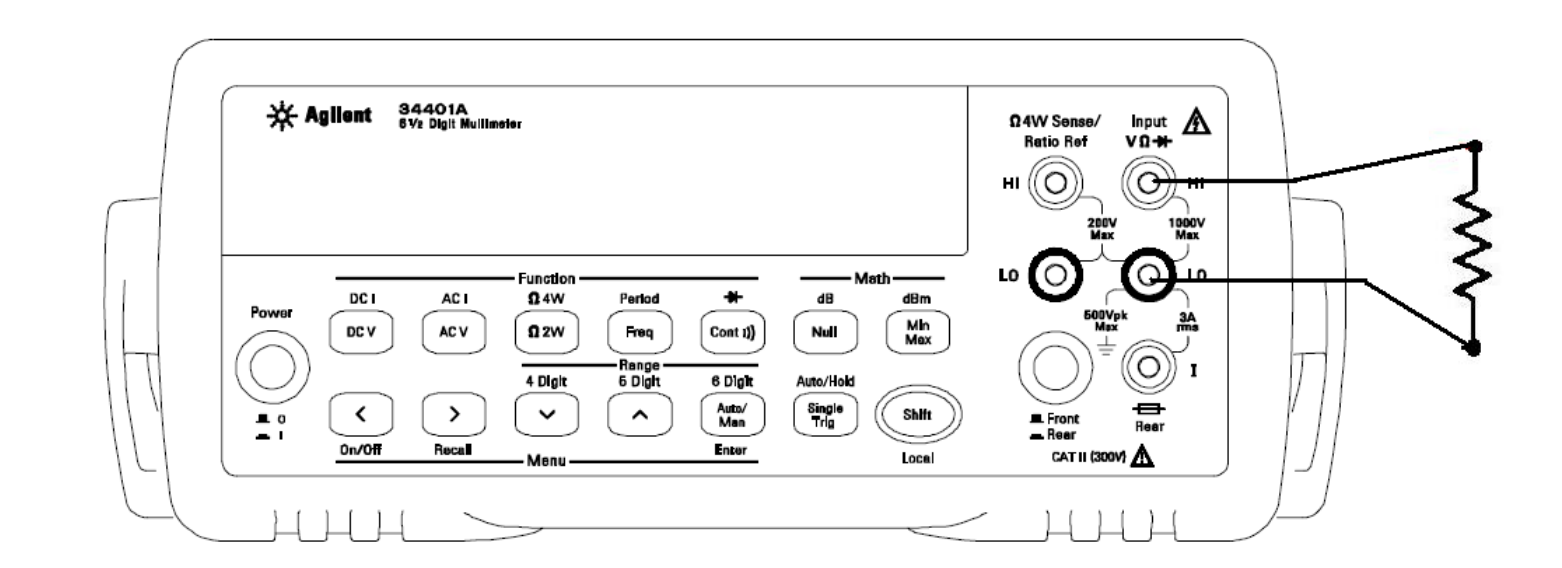
\includegraphics[height=2cm]{Relazione/media/mult_banco.png}
    \caption{Multimetro HP Hewlett Packard 34401A}
    \label{fig:mult_banco}
\end{figure}


Il multimetro HP34401A possiede un display a 6 ½ cifre. 
Per il calcolo della resistenza di valore nominale pari a (1500 ± 7,5) m$\Omega$, impostiamo la portata dello strumento a 100,0000 $\Omega$, lo strumento a 6 ½ cifre ha un campo di misura 
pari a 1/1000000 del valore di fondo scala e quindi il passo di quantizzazione Q sar\'a: 
\begin{equation}
    Q \equiv \frac{V_F_S}{CM} \equiv \frac{10^2}{10^6} = 0,0001 \Omega
\end{equation}
Con l'incertezza di quantizzazione $U_q$ pari a:
\begin{equation}
    U_q \equiv \frac{Q}{CM} \equiv 0,00005 \Omega
\end{equation}

Quando abbiamo lavorato con il multimetro da banco, abbiamo dapprima lavorato in modalità "2 terminali" (attivata premendo la modalità "$\Omega$", e poi "2W" che ci permette di lavorare a due morsetti).

\begin{figure}[h]
    \centering
    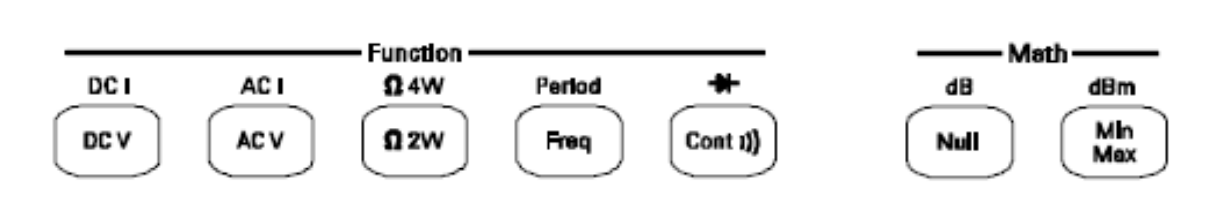
\includegraphics[height=2cm]{Relazione/media/mult_banco_zoom.png}
    \caption{Zoom sui tasti premuti}
    \label{fig:mult_banco_zoom}
\end{figure}

Come prima operazione abbiamo cortocircuitato i morsetti, premendo il tasto null, in modo che il valore di resistenza interna del conduttore dei cavi venga preso in considerazione permettendoci di tarare lo strumento, mostrando una misurazione prossima a zero (nel nostro caso abbiamo visualizzato a display, impostato a 6 cifre e mezzo, il valore 0,000134).


\begin{figure}[h]
    \centering
    \includegraphics[height=5cm]{Relazione/media/2Morsetti_432.jpg}
    \label{fig:2morsetti}
\end{figure}

\'E importante notare che se la resistenza dei cavi è comparabile o superiore alla resistenza che si desidera misurare, il risultato della misura potrebbe essere influenzato significativamente dal contributo della resistenza dei cavi, dunque per ridurre gli errori sistematici:
\begin{equation}
    Risultato = Valore letto - Valore NULL
\end{equation}

\begin{figure}[h]
    \centering
    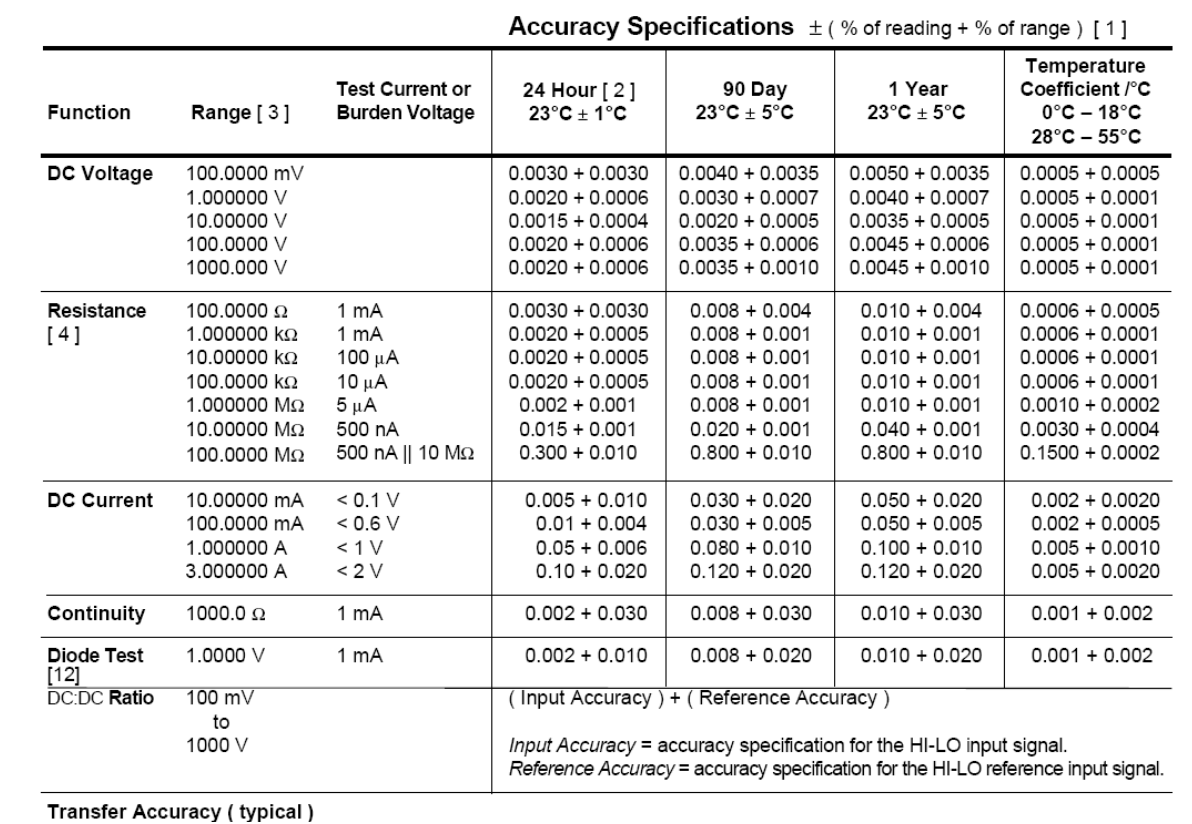
\includegraphics[height=5cm]{Relazione/media/tabella_mult_banco.png}
    \label{fig:tab_mult_banco}
\end{figure}

Avendo impostato un valore di fondo scala pari a 100,0000 $\Omega$, in un ambiente con una temperatura pari a (23 $\pm$ 5)°C, facciamo riferimento all'incertezza $\pm$(0,010 $\% \pm 0,004 \%$), con il primo termine proporzionale alla lettura e il secondo proporzionale alla portata.
Ragionando come prima, ipotizzando di unire l'incertezza di non linearità integrale nell'incertezza di portata, posso scrivere $U_g$ (incertezza di guadagno), $U_o$ (incertezza di portata dell'offset) e $U_q$ (incertezza di quantizzazione) come: 
\begin{equation}
    \left\{ \begin{array}{rcl}
| \Delta G \cdot y_q | \leq U_G |y_q|,    con U_g=0,01\%
\\ | O + inl(x) + e_q(g(x)) | \leq U_o_+_i_n_l_+_q, con U_o_+_i_n_l_+_q=0,004\%
\end{array}\right
\end{equation}
Quindi, chiamando P, portata e $V_L$ valore letto (supponiamo di usare il primo valore letto nella tabella \label{mult_port}):
\begin{equation}
    U(R) \equiv U_G \cdot V_L + U_o_+_i_n_l_+_q \cdot P \equiv 0,01\% \cdot 1,648\Omega + 0,004 \% \cdot 100 \Omega \equiv 0,004 \Omega (arrotondato per difetto)
\end{equation}

\begin{table}[h] %la h serve per metterla esattamente dove la si sta mettendo nel file in Latex
\centering
\resizebox{\textwidth}{!}{
\begin{tabular}{|c|c|c|c|c|c|cl|}
\hline
\rowcolor[HTML]{CFE2F3} 
Misure ($\Omega$) & Valore di NULL - Cortocircuito (V) & Risultato & Fondo scala ($\Omega$) & Passo Q ($\Omega$) & Incertezza Uq ($\Omega$) & \multicolumn{2}{c|}{\cellcolor[HTML]{CFE2F3}Incertezza} \\ \hline
1,648 & 0,133 & 1,515 & 100 & 0,0001 & 0,00005 & \multicolumn{2}{c|}{0,0041515} \\ \hline
1,614 & 0,133 & 1,481 & 100 & 0,0001 & 0,00005 & \multicolumn{2}{c|}{0,0041481} \\ \hline
1,627 & 0,133 & 1,494 & 100 & 0,0001 & 0,00005 & \multicolumn{2}{c|}{0,0041494} \\ \hline
1,614 & 0,133 & 1,481 & 100 & 0,0001 & 0,00005 & \multicolumn{2}{c|}{0,0041481} \\ \hline
1,432 & 0,133 & 1,299 & 100 & 0,0001 & 0,00005 & \multicolumn{2}{c|}{0,0041299} \\ \hline
1,466 & 0,133 & 1,333 & 100 & 0,0001 & 0,00005 & \multicolumn{2}{c|}{0,0041333} \\ \hline
1,441 & 0,133 & 1,308 & 100 & 0,0001 & 0,00005 & \multicolumn{2}{c|}{0,0041308} \\ \hline
1,468 & 0,133 & 1,335 & 100 & 0,0001 & 0,00005 & \multicolumn{2}{c|}{0,0041335} \\ \hline
1,475 & 0,133 & 1,342 & 100 & 0,0001 & 0,00005 & \multicolumn{2}{c|}{0,0041342} \\ \hline
1,493 & 0,133 & 1,36  & 100 & 0,0001 & 0,00005 & \multicolumn{2}{c|}{0,004136}  \\ \hline
\end{tabular}
}
\caption{Multimetro 34401A (6$\sfrac{1}{2}$ cifre), 2 Morsetti}
\label{tab:mult_2w}
\end{table}



\newline \newline \newline
 Sapendo che la resistenza misurata col multimetro è 1,648 $\Omega$, il risultato della misura si esprime come R=(+1,648 $\pm$ 0,005)$\Omega$, abbiamo operato anche con un sistema a quattro morsetti(metodo Kelvin)


\begin{figure}[h]
    \centering
    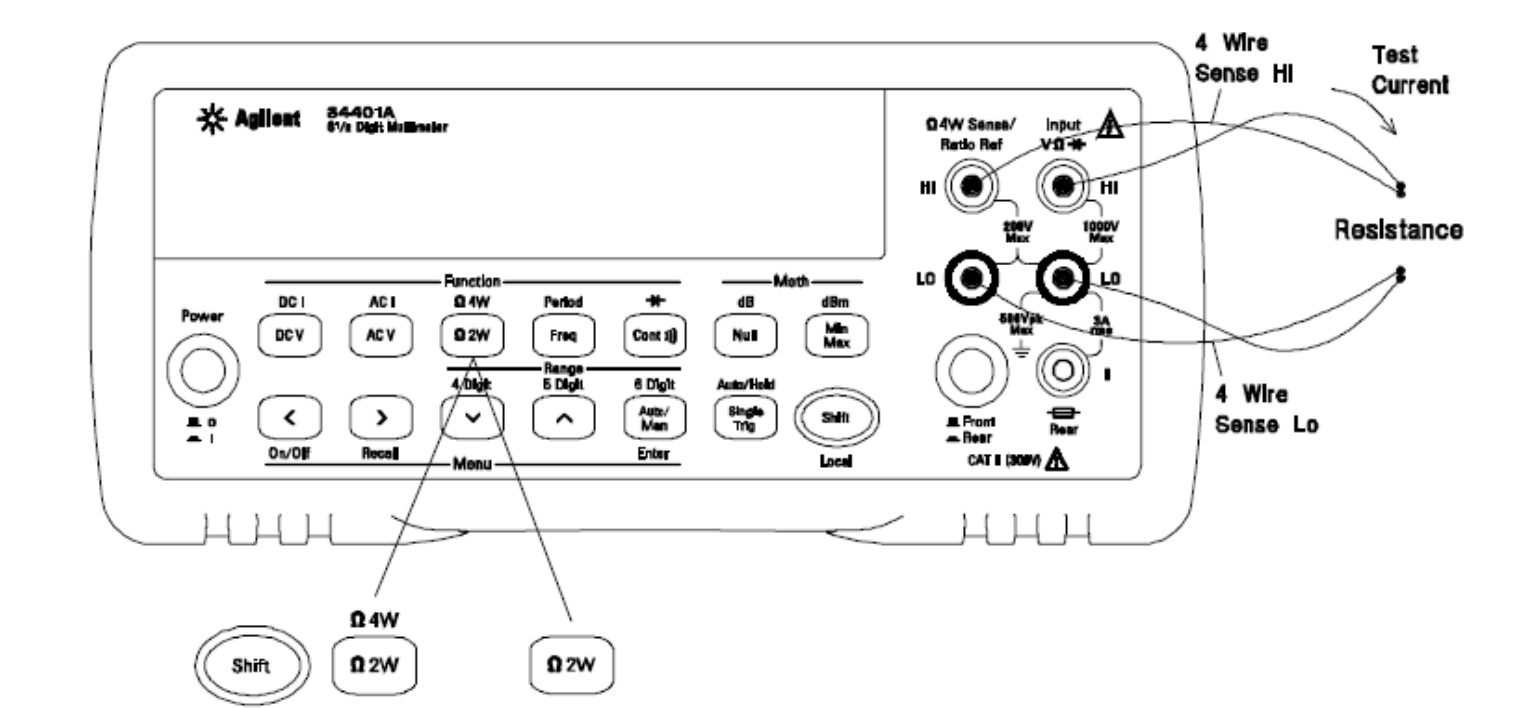
\includegraphics[height=5cm]{Relazione/media/quattro_morsetti.png}
    \caption{Metodo Kelvin a 4 morsetti}
    \label{fig:quattro morsetti}
\end{figure}





Successivamente, sempre con lo stesso multimetro da banco, abbiamo lavorato in modalità "4 terminali" (attivata sempre premendo la modalità "$\Omega$", e poi successivamente "4W" per lavorare a quattro morsetti).

\begin{figure}[h]
    \centering
    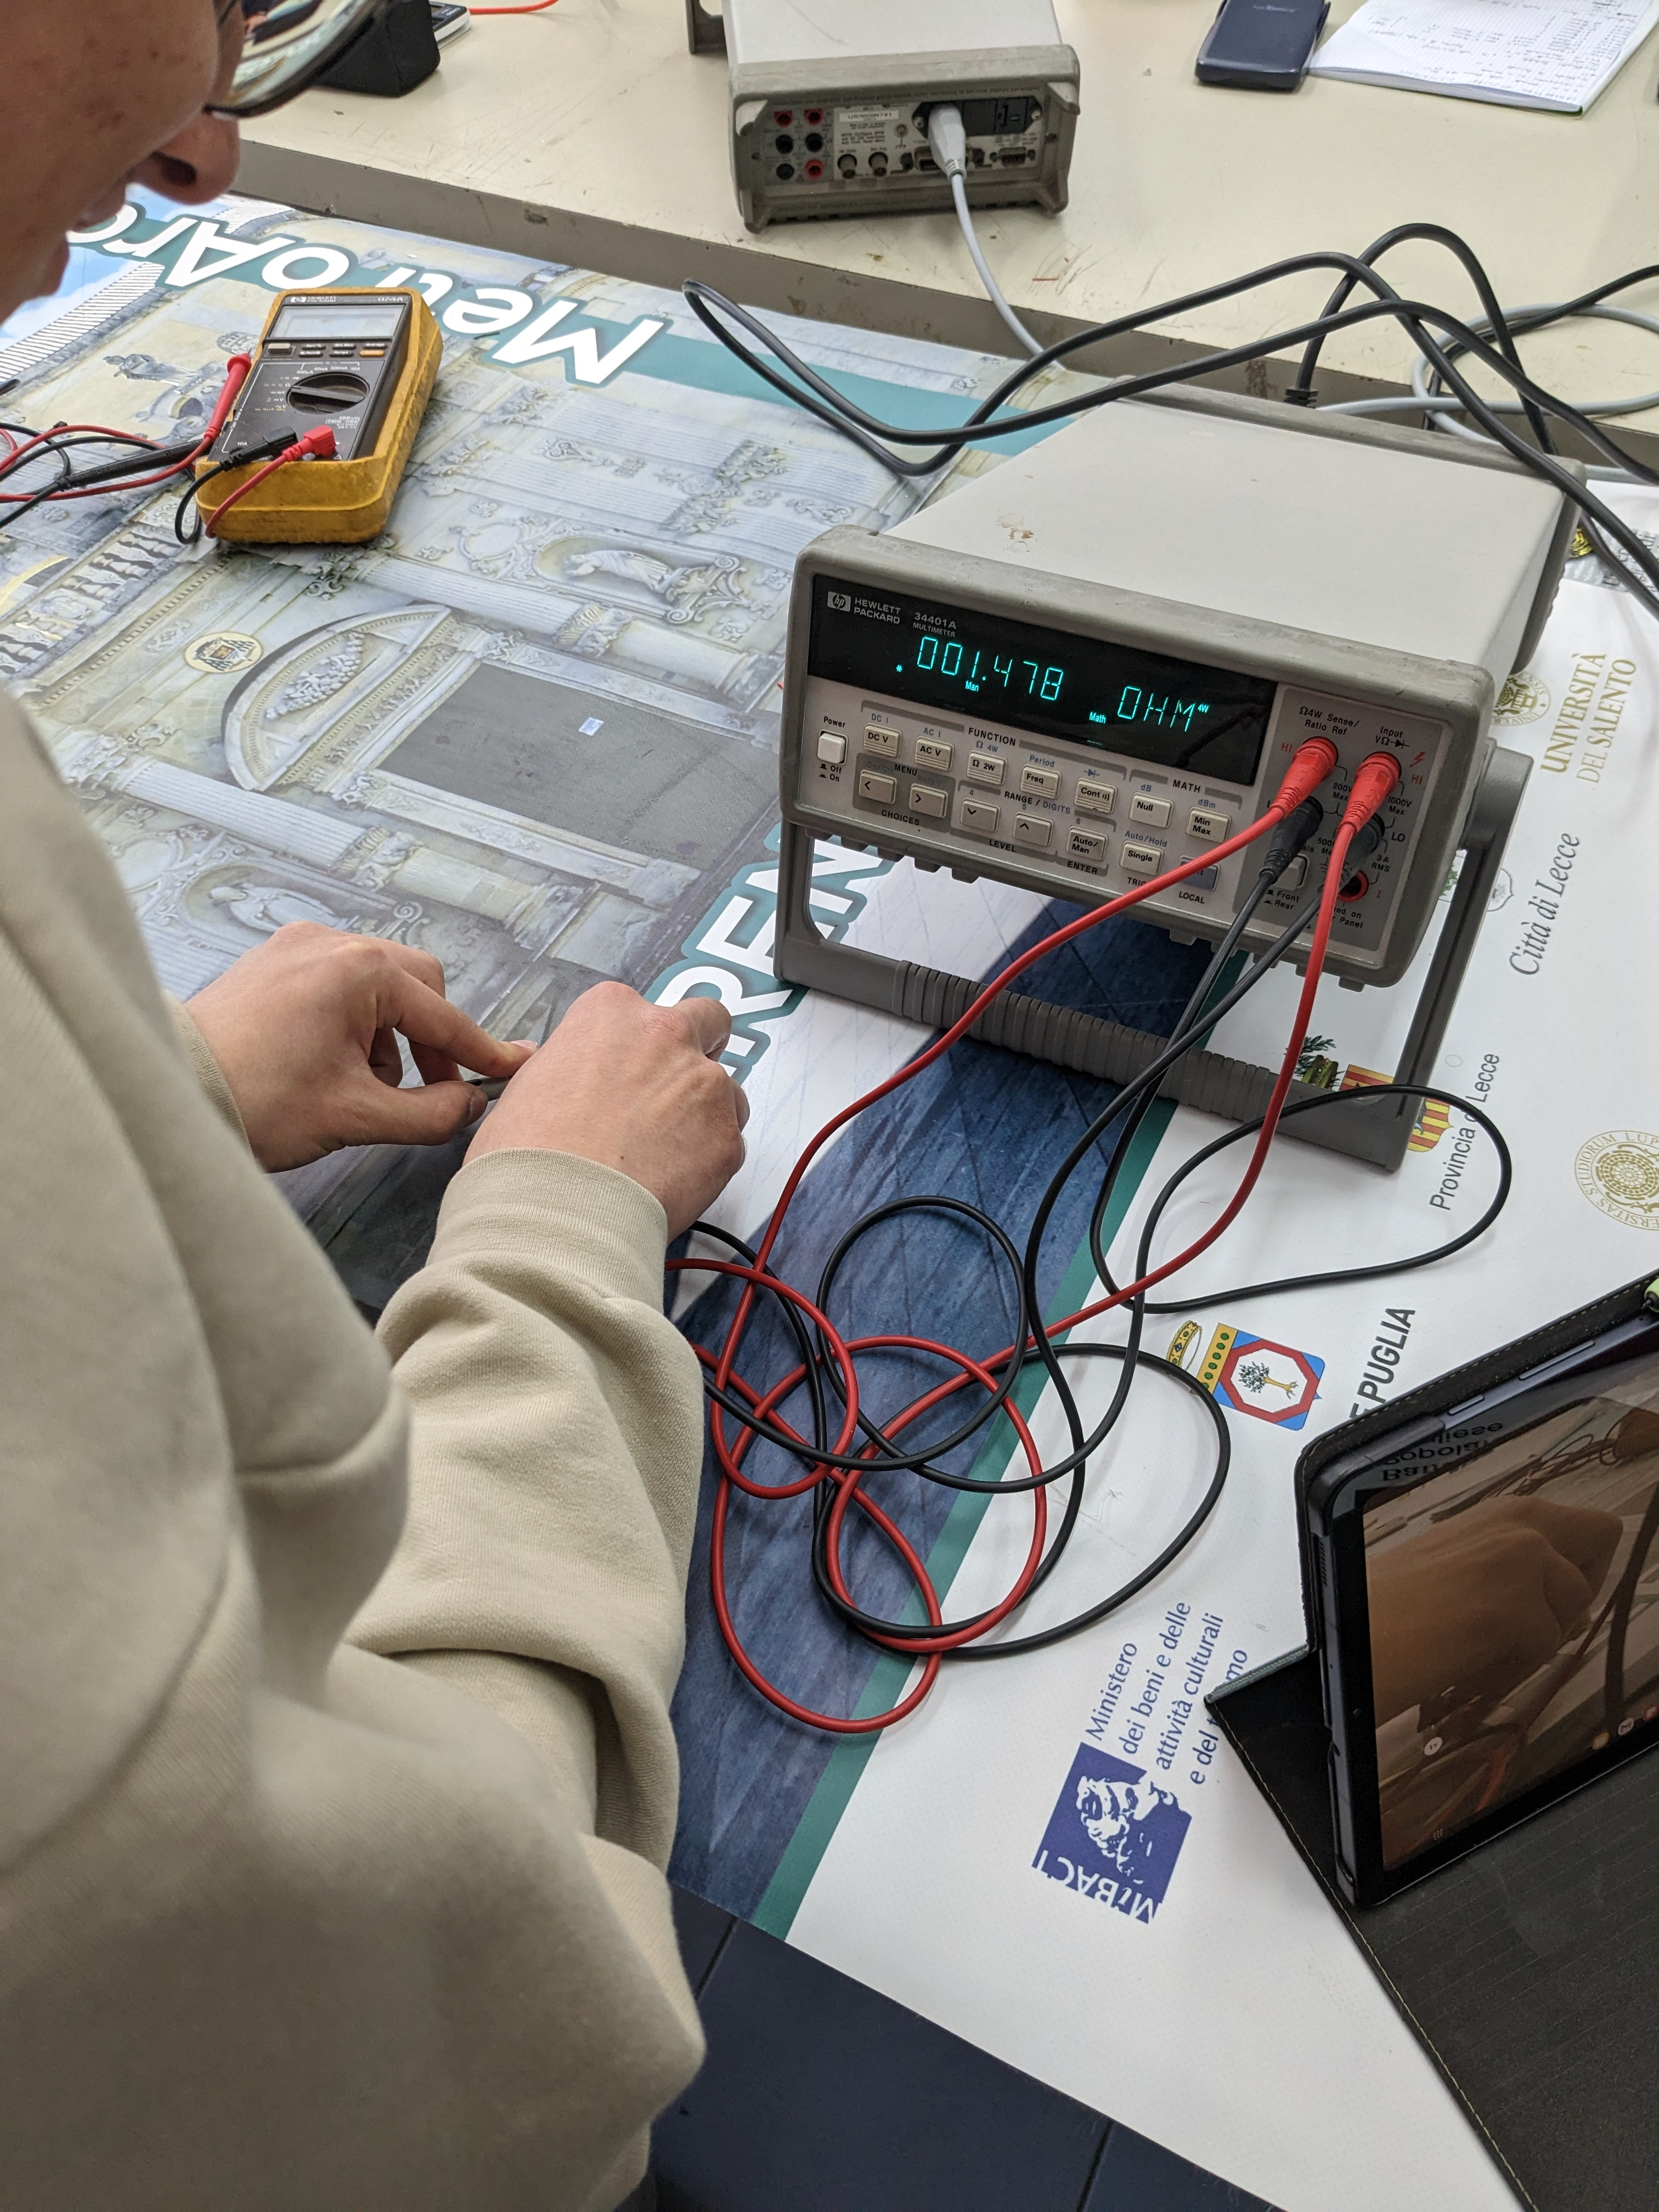
\includegraphics[height=5cm]{Relazione/media/4Morsetti_472.jpg}
    \label{fig:4morsetti}
\end{figure}
Anche in questo caso abbiamo nuovamente cortocircuitato i morsetti, premendo nuovamente il tasto null per tarare lo strumento e riavere un valore associato al cortocircuito pi\'u prossimo allo zero possibile in presenza del cortocircuito (nel nostro caso 0,004).


Attraverso la prima coppia di morsetti (Hi, Lo), lo strumento inietta la corrente nota come "$I_0$" nella resistenza. Questa corrente attraversa le boccole (Hi, Lo) dove si incontra con la resistenza di contatto, che può falsare la misura standard a due fili (impostando $\Omega$2W sul pannello frontale del multimetro).

Per evitare questo problema, tramite l'altra coppia di morsetti di sensing (Hi, Lo), viene prelevata la tensione su due punti più vicini al resistore. Utilizzando questa configurazione (impostando $\Omega$4W sul pannello frontale del multimetro), le cadute di tensione sulle resistenze di contatto presenti sulle boccole che portano la corrente al resistore in prova possono essere escluse dalla tensione da misurare, garantendo una misurazione più accurata.

Si effettua l'operazione di NULL in modo analogo al caso precedente, misurando un valore di resistenza pari a R = 1,478 Ω. Dalla teoria, questo valore dovrebbe essere più accurato rispetto al caso del multimetro a due morsetti. Utilizzando il modello precedente per il calcolo dell'incertezza, otteniamo:
\begin{equation}
    \left\{ \begin{array}{rcl}
| \Delta G \cdot y_q | \leq U_G |y_q|,    con U_g=0,01\%
\\ | O + inl(x) + e_q(g(x)) | \leq U_o_+_i_n_l_+_q, con U_o_+_i_n_l_+_q=0,004\%
\end{array}\right
\end{equation}
Quindi, chiamando P, portata e $V_L$ valore letto (supponiamo di usare il primo valore letto nella tabella \label{mult_port}):
\begin{equation}
    U(R) \equiv U_G \cdot V_L + U_o_+_i_n_l_+_q \cdot P \equiv 0,01\% \cdot 1,478\Omega + 0,004 \% \cdot 100 \Omega \equiv 0,004 \Omega 
\end{equation}
(dove il risultato è stato arrotondato per difetto)
Notiamo che l’incertezza in questo caso non è cambiata, con R=(+1,478 $\pm$ 0,005)$\Omega$



\begin{table}[h]
\centering
\resizebox{\textwidth}{!}{%
\begin{tabular}{|c|c|c|c|c|c|cl|}
\hline
\rowcolor[HTML]{CFE2F3} 
\multicolumn{1}{|l|}{\cellcolor[HTML]{CFE2F3}Misure ($\Omega$)} &
  \multicolumn{1}{l|}{\cellcolor[HTML]{CFE2F3}Valore di NULL (V) ??} &
  \multicolumn{1}{l|}{\cellcolor[HTML]{CFE2F3}Risultato} &
  \multicolumn{1}{l|}{\cellcolor[HTML]{CFE2F3}Fondo scala ($\Omega$)} &
  \multicolumn{1}{l|}{\cellcolor[HTML]{CFE2F3}Passo Q ($\Omega$)} &
  \multicolumn{1}{l|}{\cellcolor[HTML]{CFE2F3}Incertezza Uq ($\Omega$)} &
  \multicolumn{2}{l|}{\cellcolor[HTML]{CFE2F3}Incertezza} \\ \hline
1,478 & 0,004 & 1,474 & 100 & 0,0001 & 0,00005 & \multicolumn{2}{c|}{0,0041474} \\ \hline
1,478 & 0,004 & 1,474 & 100 & 0,0001 & 0,00005 & \multicolumn{2}{c|}{0,0041474} \\ \hline
1,478 & 0,004 & 1,474 & 100 & 0,0001 & 0,00005 & \multicolumn{2}{c|}{0,0041474} \\ \hline
1,478 & 0,004 & 1,474 & 100 & 0,0001 & 0,00005 & \multicolumn{2}{c|}{0,0041474} \\ \hline
1,478 & 0,004 & 1,474 & 100 & 0,0001 & 0,00005 & \multicolumn{2}{c|}{0,0041474} \\ \hline
1,478 & 0,004 & 1,474 & 100 & 0,0001 & 0,00005 & \multicolumn{2}{c|}{0,0041474} \\ \hline
1,478 & 0,004 & 1,474 & 100 & 0,0001 & 0,00005 & \multicolumn{2}{c|}{0,0041474} \\ \hline
1,478 & 0,004 & 1,474 & 100 & 0,0001 & 0,00005 & \multicolumn{2}{c|}{0,0041474} \\ \hline
1,478 & 0,004 & 1,474 & 100 & 0,0001 & 0,00005 & \multicolumn{2}{c|}{0,0041474} \\ \hline
1,478 & 0,004 & 1,474 & 100 & 0,0001 & 0,00005 & \multicolumn{2}{c|}{0,0041474} \\ \hline
\end{tabular}%
}
\caption{Multimetro 34401A (6$\sfrac{1}{2}$ cifre), 4 Morsetti}
\label{tab:mult_4w}
\end{table}




\newline \newline \newline

Osserviamo questa volta che utilizzando il multimetro da banco a 6 ½ cifre si ottiene una stima più precisa del valore misurato rispetto all'utilizzo del multimetro portatile descritto precedentemente. Questi miglioramenti possono essere attribuiti alla capacità dello strumento da banco di ridurre gli errori sistematici mediante l'implementazione di funzioni adeguate.

Il multimetro da banco a 6 ½ cifre offre una maggiore precisione grazie alla sua elevata risoluzione e alla possibilità di compensare gli errori sistematici tramite funzioni avanzate di calibrazione e correzione. Ciò consente di ottenere misurazioni più accurate e affidabili, riducendo l'effetto degli errori di offset, delle non linearità e di altri fattori che potrebbero influenzare la precisione della misura.

Inoltre, lo strumento da banco può offrire un controllo più preciso delle condizioni operative, come la compensazione della resistenza dei cavi o la selezione della modalità di misura più adatta alle specifiche dell'applicazione. Ciò contribuisce ulteriormente a migliorare l'accuratezza complessiva della misurazione.

In conclusione, usando una resistenza con valore nominale di (1500 ± 7,5) m$\Omega$, con il multimetro da banco otteniamo una stima pari a R=(+1,648 $\pm$ 0,005)$\Omega$ per la misurazione a due morsetti, mente otteniamo una stima pari a R=(+1,478 $\pm$ 0,005)$\Omega$ per la misurazione a 4 morsetti.

\begin{figure}[h]
    \centering
    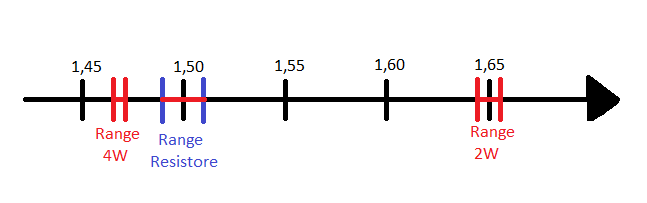
\includegraphics[height=3cm]{Relazione/media/banco_misure.png}
    \label{fig:range}
\end{figure}

eeeeeeeeeeeeeeeeeeeeeeeeeeeeeeeeeeeeeeeeeee doveva uscire che i 4w stava dentro il range del resistore, non so se dovremmo commentare o no la cosaaaaaaaaaaaaaaaaaaaaaaaaaaaaaaaaaaaaa
\newline
Volendo quantificare gli errori sistematici:
\begin{equation}
    E_S_(_2_W_) \equiv 1,648 - 1,500 = 0,148 \Omega
\end{equation}
\begin{equation}
    | E_S_(_4_W_) | \equiv | 1,478 - 1,500  |= 0,022 \Omega
\end{equation}
che portano alle seguenti accuratezze: 
\begin{equation}
    a_(_2_W_) \equiv 1 - | \frac{E_S_(_2_W_)}{R_N_O_M_I_N_A_L_E} | \equiv 91\%
\end{equation}
\begin{equation}
    a_(_4_W_) \equiv 1 - | \frac{E_S_(_4_W_)}{R_N_O_M_I_N_A_L_E} | \equiv 91\%
\end{equation}

AIUTOOOOOOOOOOOOOOO dovrebbero essere percentuali pi§ alte del multimetro da banco














%----------LCR-----------%
\section{Misure con LCR-Meter}
\label{sec:lcr}

COSè IL LCR METER (INTRODUZIONEEEEEEEEEEEEEEEEEEEEEEEEEEEEEEEEEEEEEEEEEEEEEEEEEEEEEEEEEEEEEEEEEEEEEEEEEEEEEEEEEEEEEEEEEE) + FOTOOOOOOOOOOOOOOOOOOOOO


\subsection{Impedenze}
\label{sub:z}

Tramite l'LCR-Meter abbiamo svolto l'ultima parte della nostra prima esperienza.
Innanzitutto abbiamo calibrato lo strumento per compensare gli errori sistematici introdotti dallo strumento stesso, dando come riferimento due carichi noti (il circuito virtualmente chiuso e aperto), premendo sul tassto blu dello strumento e aspettando la dicitura "short correction complete".
Per fare la prova, abbiamo avuto la possibilità di impostare vari valori di frequenza a partire da 100Hz, abbiamo impostato un tempo di misura medio ??? e impostato il modello capacità ideale con collegamento parallelo (premendo in successione i tasti CP-D e CP-RP).
Partiamo con i 100Hz, e misuriamo la resistenza (R) e reattanza (X, nel nostro caso leggermente negativà perché prevale l'effetto induttivo). Abbiamo fatto così per ogni valore della frequenza presente nella seguente tabella.  


\begin{table}[ht]
\centering
\resizebox{\textwidth}{!}{%
\begin{tabular}{|c|c|c|}
\hline
\rowcolor[HTML]{CFE2F3} 
\textit{Frequenza {[}Hz{]}} & R {[}$\Omega${]} & X {[}m$\Omega${]} \\ \hline
100Hz                       & 1,4630    & -0,04      \\ \hline
120Hz                       & 1,4628    & -0,05      \\ \hline
1kHz                        & 1,4625    & -0,52      \\ \hline
10kHz                       & 1,4622    & -5,12      \\ \hline
100kHz                      & 1,4635    & -51,50     \\ \hline
\end{tabular}%
}
\caption{LCR, misura Impedenza, Tempo di misura: Long}
\label{tab:lcr_z}
\end{table}

\begin{table}
\centering
\resizebox{\textwidth}{!}{%
\begin{tabular}{|c|c|c|c|c|c|c|c|}
\hline
\rowcolor[HTML]{CFE2F3} 
A      & B      & C & D {[}$\Omega${]} & E {[}$\Omega${]} & Zs {[}$\Omega${]} & Zx {[}$\Omega${]} & Uz (Ae) \\ \hline
0,005  & 0,0009 & 1 & 0,01      & 2,80E+08  & 1          & 1,4630     & 0,0125  \\ \hline
0,005  & 0,0009 & 1 & 0,01      & 2,80E+08  & 1          & 1,4628     & 0,0125  \\ \hline
0,004  & 0,0003 & 1 & 0,0165    & 2,80E+07  & 1          & 1,4625     & 0,0155  \\ \hline
0,004  & 0,0003 & 1 & 0,075     & 2,80E+06  & 1          & 1,4622     & 0,0555  \\ \hline
0,0097 & 0,0011 & 1 & 0,75      & 2,80E+05  & 1          & 1,4635     & 0,5229  \\ \hline
\end{tabular}%
}
\caption{Tabella di incertezza fornita dal costruttore, con Uz l'incertezza}
\label{tab:lcr_z_sheet}
\end{table}



%-------------Capacità----------- NON CAPISCO PERCHé LA METTE PRIMA DELLE TABELLE #*+ç-*°à°°àààAAAAAAAAAAAAAAAAAAAAAAAAAAAAAAAAAAAAAAAAAAAAAA%
\subsection{Capacità}
\label{sub:c}
Come ultima parte della prova abbiamo misurato la capacità del condensatore.
Premiamo in successione "CP" (capacità), "RP" (resistenza parallela) e poi "D" (per il valore della tangente dell'angolo di perdita). Questa procedura è stata ripetuta per tutti i valori di frequenza (partendo da 100kHz, arrivando fino ai 100Hz).


\begin{table}[ht]
\centering
\caption{LCR, misura della capacità}
\label{tab:lcr_c}
\end{table}





    
    %\hypersetup{hidelinks}
    %\chapter{Misure di resistenza con multimetro da banco}
\label{chap:mult}

    
    %\hypersetup{hidelinks}
    %\chapter{Misure di impedenze con LCR-Meter}
\label{chap:lcr}
    
    % Chapter 3
    \hypersetup{hidelinks}
    \chapter{Compensazione in frequenza di una sonda  e Caratterizzazione di un filtro RC}
\label{chap:seconda_prova}

\section*{Obbiettivo}
L'obbiettivo della seconda esperienza di laboratorio è quello di effettuare la compensazione in frequenza di una sonda e poi di ricavare i diagrammi di Bode di un filtro passabasso passivo RC, i valori di \emph{attenuazione} e \emph{sfasamento} con le relative \emph{incertezze} mediante valutazioni di tipo B.

\section{Compensazione in frequenza di una sonda}
Le sonde costituiscono un componente fondamentale per poter prelevare un
segnale da osservare e da trasferire poi allo strumento.

\begin{figure}[h]
    \centering
    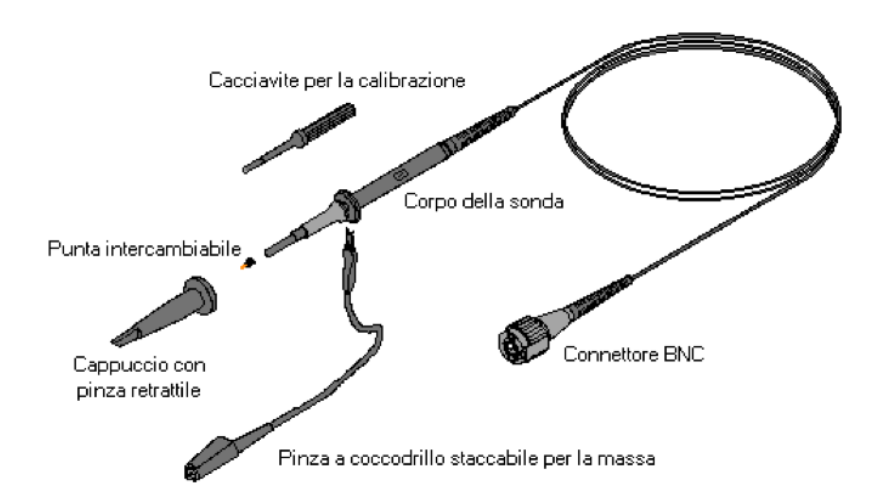
\includegraphics[height=7cm]{sonda.png}
    \caption{Sonda}
    \label{fig:sonda}
\end{figure}

La sonda può essere schematizzata in maniera semplificata come un parallelo di una resistenza e una capacità variabile. L'oscilloscopio d'altra parte ha una certa capacità intrinseca in parallelo ad una resistenza di ingresso. Tale capacità in regime AC può essere un problema, in quanto all'aumentare della frequenza inizia ad agire come un filtro passa-basso.

Per questo motivo è necessario effettuare la \textbf{compensazione in frequenza della sonda}, cioè impostare il valore della capacità variabile della sonda per andare a compensare gli effeti della capacità di ingresso dell'oscilloscopio, quindi da rendere il sistema sonda+oscilloscopio indipendente dalla frequenza.

\subsection*{}
Per poter effettuare la compensazione, abbiamo collegato il connettore BNC della sonda al canale 1 dell'oscilloscopio. Abbiamo poi sollevato il cappuccio della sonda e l'abbiamo collegata all'occhiello presente nella parte inferiore del dispositivo, che risulta essere la sorgente di onda quadra di ampiezza 5V e frequenza 1.2KHz generata dall'oscilloscopio stesso.

Poichè la sonda fornisce un'attenuazione pari a 10, premendo sul tasto 1 della sezione verticale, è possibile impostare il valore di \emph{Probe} su 10, mediante il tasto presente sotto lo schermo, in modo che la lettura sia riferita all'attenuazione implicita della sonda.

Fatto ciò abbiamo sistemato i valori di $K_v$ e $K_t$ per visualizzare circa 2 periodi e in modo ottimale sullo schermo l'onda quadra.

Abbiamo infine utilizzato un cacciavite in prossimità del corpo della sonda, per regolare la capacità variabile, finchè il segnale visualizzato non è apparso quanto più rettangolare possibile rispetto alla condizione iniziale in cui erano presenti delle sovra-elongazioni dovute alla sovracompensazione.


\clearpage
\section{Caratterizzazione di un Filtro RC} \label{sec:filtroRC}
Nel seguente paragrafo verrà descritto in breve il filtro RC e le sue caratteristiche. Seguirà una presentazione della strumentazione utilizzata, la descrizione della configurazione dei dispositivi e la procedura di misura.

\subsection{Filtro RC}
Il filtro RC è un sistema che effettua sul suo segnale di ingresso una funzione di attenuazione in quanto filtro passivo, cioè composto da componenti passivi quali un condensatore e un resistore in serie.

\begin{figure}[h]
    \centering
    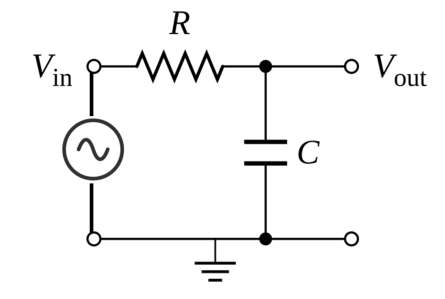
\includegraphics[height=5cm]{filtroRC.png}
    \caption{Filtro RC}
    \label{fig:filtroRC}
\end{figure}
\FloatBarrier

Esso è un filtro passa basso che cioè permette il passaggio delle frequenze al di sotto di una \textbf{frequenza di taglio} e attenua invece quelle alte. In particolare, l'attenuazione $A$ del filtro RC è definita come:

\[A=\frac{V_o}{V_i}=\frac{1}{1+j\omega RC}\]

La frequenza di taglio del filtro è definita come la frequenza alla quale la potenza del segnale in uscita dal filtro è pari alla metà della potenza del segnale in ingresso ad esso. Oppure è definita come la frequenza alla quale la tensione disponibile in uscita è $1/\sqrt{2}$ la tensione di ingresso disponibile in banda passante.

La frequenza di taglio \emph{teorica} si calcola uguagliando il modulo dell'attenuazione $A$ al valore $1/\sqrt{2}$

\[\frac{1}{\sqrt{1+(\omega RC)^2}} = \frac{1}{\sqrt{2}}\]
\[1+(\omega RC)^2 = 2\] 
\[(\omega RC)^2 = 1\]
\[\omega ^2 = \frac{1}{(RC)^2}\]
Ricordando che $\omega = 2\pi f$, si ha che la frequenza di taglio è pari a 
\[f=\frac{1}{2\pi RC}\]

\subsection{Strumentazione utilizzata}
\subsection*{PCB}
Il PCB (Printed Circuit Board) è una scheda elettronica fornita durante l'esercitazione, sulla quale, mediante l'utilizzo di jumper come nella configurazione in Figura \ref{fig:pcb_rc}, è stato realizzato un filtro RC, i cui valori di resistenza e capacità sono rispettivamente 10k$\Omega$ e 47nF.

\begin{figure}[h]
    \centering
    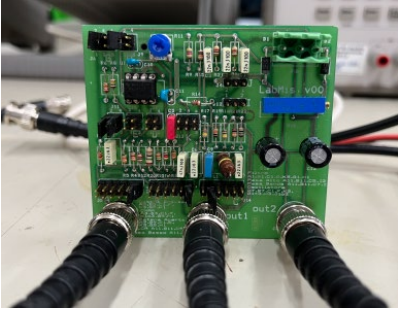
\includegraphics[width=0.9\linewidth, height=8cm]{PCB.png} 
    \caption{PCB}
    \label{fig:pcb}
\end{figure}

\begin{figure}[h]
    \centering
    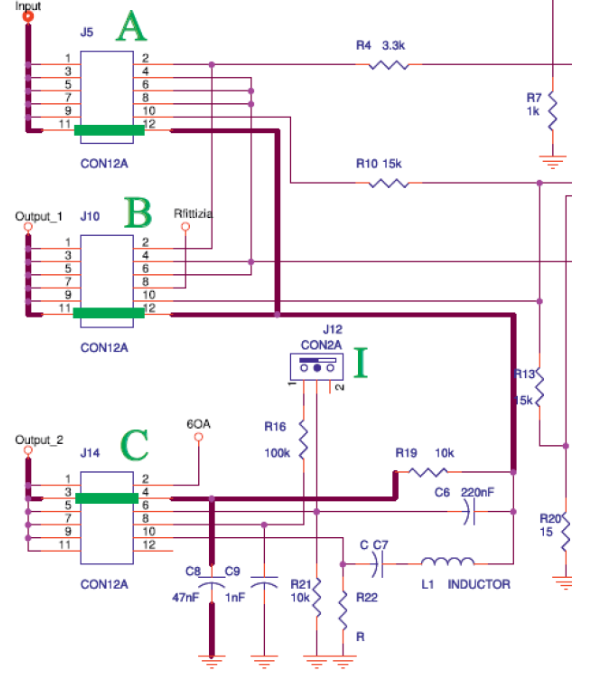
\includegraphics[width=0.9\linewidth, height=14cm]{PCB_RC.png}
    \caption{Configurazione di filtro RC del PCB}
    \label{fig:pcb_rc}
\end{figure}
\FloatBarrier

\clearpage
\subsection*{Oscilloscopio Agilent Hp 54600B}
\begin{figure}[h]
    \centering
    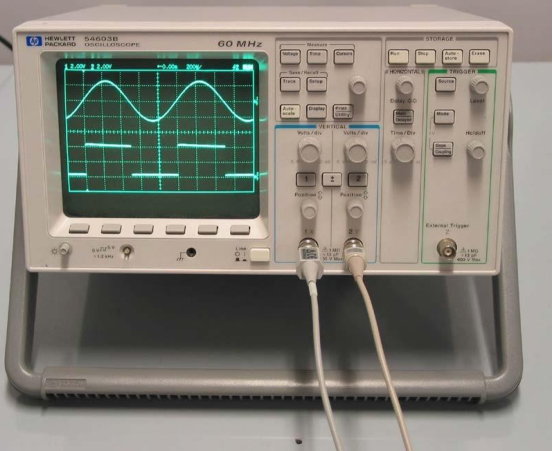
\includegraphics[width=0.9\linewidth, height=9cm]{oscill.png}
    \caption{Oscilloscopio Agilent Hp 54600B}
    \label{fig:oscill}
\end{figure}
\FloatBarrier

\subsection*{Generatore di funzioni Agilent 33120B}
\begin{figure}[h]
    \centering
    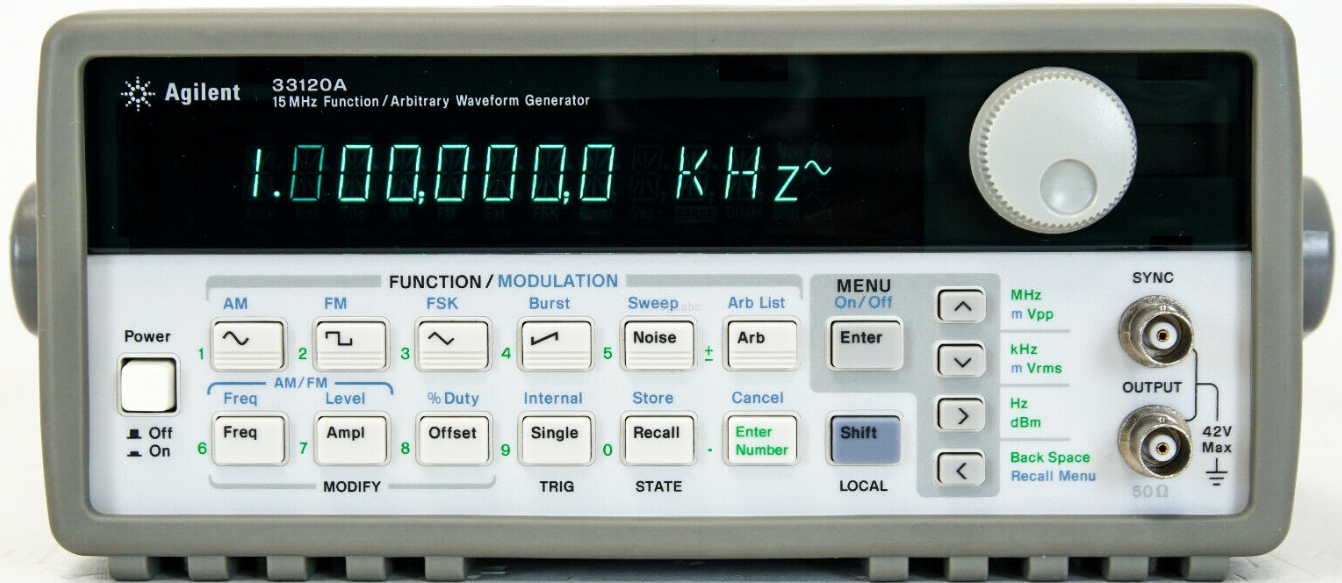
\includegraphics[width=\linewidth, height=6cm]{gen_fun.png}
    \caption{Generatore di funzioni Agilent 33120B}
    \label{fig:gen_fun}
\end{figure}
\FloatBarrier

\subsection*{Cavi di connessione (BNC-BNC)}
\clearpage

\subsection{Configurazione della strumentazione per la misurazione}

Prima di iniziare ad effettuare le misurazioni del caso, abbiamo configurato tutte le strumentazioni a disposizione. Abbiamo dunque:

\begin{itemize}
    \item Collegato i cavi di connessione secondo la seguente configurazione:
    \begin{itemize}
        \item Uscita del generatore di funzioni all'ingresso (BNC INPUT) del filtro RC
        \item Ingresso del filtro RC (BNC OUTPUT 1) al canale 1 dell'oscilloscopio
        \item Uscita del filtro RC (BNC OUTPUT 2) al canale 2 dell'oscilloscopio
    \end{itemize}
    \begin{figure}[h]
        \centering
        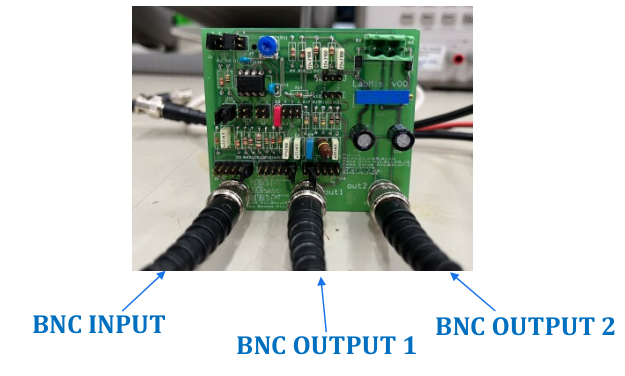
\includegraphics{PCB_bnc.png}
        \caption{Ingressi/Uscite del filtro RC}
        \label{fig:pcb_bnc}
    \end{figure}
    \begin{figure}[h]
        \centering
        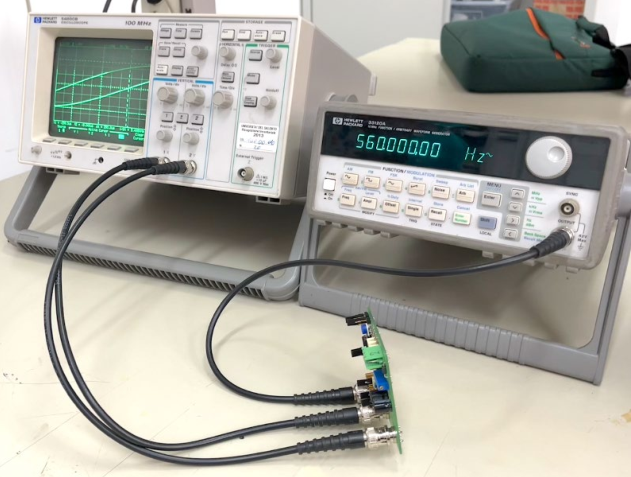
\includegraphics[width=0.9\linewidth, height=6.5cm]{conf_bnc.png}
        \caption{Configurazione dei cavi di connessione}
        \label{fig:conf_bnc}
    \end{figure}
    \FloatBarrier

    \item Avviato il generatore di funzioni impostando una frequenza iniziale di 100kHz mediante il tasto \emph{Freq} e impostato una forma d'onda sinusoidale di ampiezza pari a 5 V.
    
    \'E importante osservare che l'ampiezza visualizzata sull'oscilloscopio è diversa da quella impostata sul generatore di funzioni a causa del disattamento di impedenza tra l'oscilloscpio ed il generatore di funzioni. In particolare, in corrispondenza della tensione picco-picco di 5 V impostata per l'ingresso del filtro, verrà visualizzata una tensione picco-picco di 10 V sul display dell'oscilloscopio.
    \item Avviato l'oscilloscopio su cui visualizzare il segnale d'ingresso del filtro $V_i$ sul canale 1, e il segnale di uscita del filtro $V_o$ sul canale 2.
    Poichè abbiamo utilizzato cavi BNC-BNC e non sonde, abbiamo impostato il valore di \emph{Probe} a 1 mediante l'apposito pulsante posto sotto lo schermo.
    Per migliorare la visualizzazione di entrambi i segnali, abbiamo premuto il pulsante \emph{Auto-Scale}, che permette all'oscilloscopio di visualizzare entrambi i segnali, uno per ognuno della due metà dello schermo.
    
    Ai fini delle misurazioni da effettuare, abbiamo impostato entrambe le forme d'onda sulla linea di 0 V secondo la seguente procedura per entrambi i canali:
    \begin{enumerate}
        \item Selezione del singolo canale dal rispettivo pulsante della sezione verticale
        \item Impostazione del \emph{Coupling} su Ground mediante il secondo pulsante posizionato sotto lo schermo
        \item Utilizzo della manopola presente sotto la sezione Measure per spostare il riferimento del segnale sulla linea di 0 V
        \item Impostazione del \emph{Coupling} su AC mediante il secondo pulsante posizionato sotto lo schermo  
    \end{enumerate}
\end{itemize}

\clearpage


\subsection{Misurazioni}

\subsubsection{Calcolo della frequenza di taglio sperimentale}

Come definito nel paragrafo introduttivo sul filtro RC (\ref{sec:filtroRC}), la frequenza di taglio teorica è pari a
\[f=\frac{1}{2\pi RC}= \frac{1}{2\pi \cdot10^4 \cdot 47 \cdot10^{-9}} = 338,627 Hz\]
Questa tuttavia non sarà mai pari a quella effettiva, pertanto abbiamo ricavato sperimentalmente la frequenza di taglio effettiva. Poichè il segnale in ingresso era pari a 5 V, visualizzati 10V sull'oscilloscopio, la frequenza di taglio è quella frequenza in corrispondenza della quale l'uscita $V_{o}$ del filtro è pari a 
\[\frac{10}{\sqrt{2}} = 7,07 V\]

Abbiamo allora premuto prima sul pulsante \emph{Cursors}, selezionato il cursore $V_1$ posizionandolo per mezzo della mapanopola ad un valore di 3,5 V, 
e il cursore $V_2$ posizionandolo ad un valore di -3,5 V. In questo modo la distanza tra i due cursori era pari a 7 V.

Andando quindi ad operare sul genereatore di funzioni, abbiamo modificato la frequenza del segnale in ingresso al filtro finché il segnale di uscita (canale 2) non appariva esattamente tangente ai due cursori precedentemente posizionati.
La frequenza per cui tale condizione è soddisfatta corrisponde alla frequenza di taglio reale del filtro che è pari a 
\[f_{sperimentale} = 338,63Hz\]

In base al datasheet del generatore di funzioni, il valore dell'incertezza relativa di caso peggiore per misure di frequenza è di 20 ppm (parti per milione), cioè 
\[U_{r,f} = 20 ppm\]
L'incertezza di caso peggiore sarà pari a
\[U_f = 338 Hz\cdot U_{r,f} = 338,63Hz \cdot 20 \cdot 10^{-6} = 6,773\cdot10^{-3}Hz\]


\clearpage
\subsubsection{Misure di tensione picco-picco e $\Delta t$}

Per riuscire a ricavare i diagrammi di Bode dell'attenuazione A del filtro RC, è stato necessario ripetere la stessa procedura di misura, lasciando invariate le condizioni operative, per un totale di 17 diversi valori di frequenza.

Per ogni misurazione abbiamo quindi eseguito i seguenti passi:
\begin{enumerate}
    \item Impostato il valore della frequenza del segnale di ingresso del filtro  sul generatore di funzioni, premendo prima il pulsante \emph{Freq} e poi impostando la frequenza desisderata.
    \item Regolato i valori di $K_{V_i}$ e $K_{V_o}$ mediante le manopole poste nella parte superiore della sezione verticale, in modo da coprire quanto più possibile lo schermo senza tagliare la forma d'onda. In questo modo le misure eseguite sono più accurate e viene ridotta l'incertezza di misura.
    \item Regolato il valore di $K_t$ mediante l'apposita manopola posta nella sezione orizzontale per migliorare la visualizzazione dei segnali.
    \item Premuto il pulsante \emph{Voltage}, situato nella sezione \emph{Measure} e selezionato per ognuno dei due segnali il tipo di misura, cioè tensione picco-picco $V_{p-p}$, mediante gli appositi pulsanti posizionati sotto lo schermo.
    In questo modo i valori di tensione picco-picco di entrambi i segnali vengono automaticamente calcolati dall'oscilloscpio e visualizzati nella parte inferiore dello schermo.
    \item Premuto il pulsante \emph{Cursors} e selezionato i cursori verticali $t_1$ e $t_2$, dagli appositi pulsanti posti sotto lo schermo. Ciascun cursore , mediante la manopola presente sotto la sezione \emph{Measure}, è stato poi collocato in corrispondenza dei punti in cui il corrispondente segnale passava per lo zero. Il valore $\Delta t$  calcolato dall'oscilloscopio è poi visualizzato nella parte inferiore dello schermo. 
    
\end{enumerate}

% scrivere le formuke usate per ricavare incertezze ib ase ai datasheet
% piccolo excursus su cosa sono quei valori
% mettere tabelle di excel

\clearpage

\subsection{Calcolo delle incertezze}
In questo paragrafo si effettuerà sulle misure ottenute la valutazione dell'incertezza di \textbf{tipo B}, basata sull'utilizzo di informazioni note a priori quali le specifiche metrologiche degli strumenti adoperati.

\subsubsection{Misure Dirette}

Le misure dirette effettuate durante l'esperienza di laboratorio sono le seguenti:
\begin{itemize}
    \item \textbf{tensione picco-picco V}
    \item \textbf{distanza temporale $\Delta t$}  fra i segnali sinusoidali $V_i$ e $V_o$
    \item \textbf{freqeunza f} dei segnali $V_i$ e $V_o$ 
\end{itemize}


\subsubsection*{Incertezza associata alle misure di tensione picco-picco V}

Dalle specifiche metrologiche di ampiezza dell'oscilloscopio, poichè abbiamo utilizzato i due cursori orizzontali per le misure, consideriamo la \textbf{Dual cursor accuracy}, pari a 
\[vertical \ accuracy \pm 0.4\% \ of full scale\]

dove \textbf{vertical accuracy} per l'oscilloscopio Agilent HP 54600B è pari a 1.9\%, mentre \textbf{full scale} è il fondo scala del dispositivo ed è pari a $y_{FS} = 8 \cdot k_v$, dove 8 sono le divisioni verticali e $k_v$ è la \emph{vertical sensitivity} espressa in V/div.

La \emph{Dual cursor accuracy} sopra riportata deriva dalla formula generale dell'incertezza per una differenza 
\[U(V_1 - V_2) = U_G|V_1 - V_2| + 2U_{inl} + 2U{q}\]

Nel nostro caso, l'incertezza di non linearità integrale $U_{inl}$, è stata conglobata nel termine 1.9\% insieme a $U_G$ incertezza di guadagno. L'incertezza di quantizzazione $2U_q$ è invece pari al termine $\pm 0.4\% \cdot y_{FS}$. L'incertezza di offset $U_O$ non è presente poichè nel caso di differenze di misure l'errore di offset si compensa.

Indicato quindi con $V$ il valore di tensione picco-picco letto, l'\textbf{incertezza di caso peggiore} associata a $V$ è data dalla seguente formula:

\[U_V = \frac{1.9}{100} \cdot |V| + \frac{0.4}{100} \cdot 8 \cdot k_v\]

Da questa formula è possibile poi ricavare l'\textbf{incertezza relativa di caso peggiore}:
\[U_{r,V} = \frac{U_V}{V}\]

Seguono due tabelle contenenti per ogni valore di frequenza: il valore di tensione letto, la vertical sensitivity all'atto della lettura, l'incertezza assoluta di caso peggiore e l'incertezza relativa di caso peggiore.

\begin{table}[!ht]
    \centering
    \begin{tabular}{|c|c|c|c|c|}
    \hline

        \textbf{f [Hz]} & \textbf{$\bm{V_{i}}$ [V]} & \textbf{$\bm{K_{V_i}}$ [V/div]} & \textbf{U($\bm{V_{i}}$)} & \textbf{$\bm{U_{r}}$($\bm{V_{i}}$)} \\ \hline

        1 & 3,938 & 1 & 0,1068 & 0,02713 \\ \hline
        2 & 6,468 & 1 & 0,1549 & 0,02395 \\ \hline
        3 & 7,875 & 2 & 0,2136 & 0,02713 \\ \hline
        6 & 9,375 & 2 & 0,2421 & 0,02583 \\ \hline
        10 & 9,75 & 2 & 0,2493 & 0,02556 \\ \hline
        18 & 10 & 2 & 0,2540 & 0,02540 \\ \hline
        32 & 10,12 & 2 & 0,2563 & 0,02532 \\ \hline
        56 & 10,25 & 2 & 0,2588 & 0,02524 \\ \hline
        100 & 10,12 & 2 & 0,2563 & 0,02532 \\ \hline
        180 & 10 & 2 & 0,2540 & 0,02540 \\ \hline
        320 & 9,875 & 2 & 0,2516 & 0,02548 \\ \hline
        560 & 9,75 & 2 & 0,2493 & 0,02556 \\ \hline
        1000 & 8,875 & 2 & 0,2326 & 0,02621 \\ \hline
        1800 & 9,625 & 2 & 0,2469 & 0,02565 \\ \hline
        3200 & 9,875 & 2 & 0,2516 & 0,02548 \\ \hline
        5600 & 9,875 & 2 & 0,2516 & 0,02548 \\ \hline
        10000 & 9,875 & 2 & 0,2516 & 0,02548 \\ \hline
    \end{tabular}
\end{table}

\begin{table}[!ht]
    \centering
    \begin{tabular}{|c|c|c|c|c|}
    \hline

        \textbf{f [Hz]} & \textbf{$\bm{V_{o}}$ [V]} & \textbf{$\bm{K_{V_o}}$ [V/div]} & \textbf{U($\bm{V_{o}}$)} & \textbf{$\bm{U_r}$($\bm{V_{o}}$)} \\ \hline

        1 & 4 & 1 & 0,1080 & 0,02700 \\ \hline
        2 & 6,531 & 1 & 0,1561 & 0,02390 \\ \hline
        3 & 7,875 & 2 & 0,2136 & 0,02713 \\ \hline
        6 & 9,25 & 2 & 0,2398 & 0,02592 \\ \hline
        10 & 9,635 & 2 & 0,2471 & 0,02564 \\ \hline
        18 & 9,875 & 2 & 0,2516 & 0,02548 \\ \hline
        32 & 9,938 & 2 & 0,2528 & 0,02544 \\ \hline
        56 & 10 & 2 & 0,2540 & 0,02540 \\ \hline
        100 & 9,625 & 2 & 0,2469 & 0,02565 \\ \hline
        180 & 8,75 & 2 & 0,2303 & 0,02631 \\ \hline
        320 & 7,188 & 2 & 0,2006 & 0,02790 \\ \hline
        560 & 5,125 & 2 & 0,1614 & 0,03149 \\ \hline
        1000 & 2,859 & 0,50 & 0,0703 & 0,02460 \\ \hline
        1800 & 1,797 & 0,50 & 0,0501 & 0,02790 \\ \hline
        3200 & 1,05 & 0,20 & 0,0264 & 0,02510 \\ \hline
        5600 & 0,606 & 0,10 & 0,0147 & 0,02428 \\ \hline
        10000 & 0,342 & 0,05 & 0,0081 & 0,02368 \\ \hline
    \end{tabular}
\end{table}

\FloatBarrier
\clearpage


\subsubsection*{Incertezza temporale associata alle misure di distanza temporale $\Delta t$}

Le specifiche metrologiche della base dei tempi dell'oscilloscopio forniscono la seguente espressione per la \textbf{Delta t accuracy}:

\[\pm0.01\% \pm0.2\% \ of full scale \pm 200 \ ps\]

Possiamo dare un'interpretazione dell'espressione a partire dalla formula dell'incertezza sulla differennza di misure di tempo:
\[U(T_1 - T_2) = U_S |T_1 - T_2| + 2U_{tbd} + 2U_{T_c}\]

$U_S$ incertezza sulla velocità di sweep, equivale al coefficiente $\pm0.01\%$.
$2U_{tbd}$ incertezza di distorsione della base dei tempi è pari al valore $\pm200 \ ps$.
$2U_{T_c}$ incertezza di risoluzione, equivale al termine $\pm0.2\% \ of full scale$, dove full scale è il valore di fondoscala pari a $\tau _{FS}  = 10 \cdot k_t$.
Infine, poichè si parla di differenze di misure, l'incertezza di ritardo del trigger $U_D$ è trascurabile.

Indicato con $\Delta t$ il valore di distanza temporale tra i segnali $V_i$ e $V_o$, l'\textbf{incertezza assoluta di caso peggiore} associata a $\Delta t$ è data dalla seguente formula:

\[U_{\Delta t} = \frac{0.01}{100} \cdot |\Delta t| + \frac{0.2}{100} \cdot  10 \cdot k_t + 200 \ ps  \]

Da questa formula è possibile poi ricavare l'\textbf{incertezza relativa di caso peggiore}:
\[U_{r,\Delta t} = \frac{U_{\Delta t}}{\Delta t}\]

Segue per ogni valore di frequenza: il valore di $\Delta t$ letto, il valore di $k_t$, l'incertezza (assoluta e relativa) di caso peggiore

\begin{table}[!ht]
    \centering
    \begin{tabular}{|c|c|c|c|c|}
    \hline

        \textbf{f [Hz]} & \textbf{$\bm{\Delta t}$ [µs]} & \textbf{$\bm{K_t}$ [µs/div]} & \textbf{U($\bm{\Delta t}$)} & \textbf{$\bm{U_r(\Delta t)}$} \\ \hline

        1 & 3200 & 500,00 & 0,00001032 & 0,00323 \\ \hline
        2 & 2140 & 500,00 & 0,00001021 & 0,00477 \\ \hline
        3 & 1550 & 200,00 & 0,00000416 & 0,00268 \\ \hline
        6 & 684 & 100,00 & 0,00000207 & 0,00302 \\ \hline
        10 & 592 & 100,00 & 0,00000206 & 0,00348 \\ \hline
        18 & 500 & 100,00 & 0,00000205 & 0,00410 \\ \hline
        32 & 480 & 100,00 & 0,00000205 & 0,00427 \\ \hline
        56 & 464 & 100,00 & 0,00000205 & 0,00441 \\ \hline
        100 & 448 & 200,00 & 0,00000405 & 0,00903 \\ \hline
        180 & 424 & 100,00 & 0,00000204 & 0,00482 \\ \hline
        320 & 370 & 50,00 & 0,00000104 & 0,00280 \\ \hline
        560 & 276 & 50,00 & 0,00000103 & 0,00372 \\ \hline
        1000 & 203 & 50,00 & 0,00000102 & 0,00503 \\ \hline
        1800 & 128 & 20,00 & 0,00000041 & 0,00324 \\ \hline
        3200 & 77 & 10,00 & 0,00000021 & 0,00269 \\ \hline
        5600 & 43 & 10,00 & 0,00000020 & 0,00478 \\ \hline
        10000 & 24 & 5,00 & 0,00000010 & 0,00421 \\ \hline
    \end{tabular}
\end{table}
\FloatBarrier
\clearpage


\subsubsection*{Incertezza associata alle misure di frequenza f}

Le specifiche metrologiche del generatore di funzioni, forniscono il valore dell'\textbf{incertezza relativa di caso peggiore} per le misure di frequenza, pari a :

\[U_{r,f} = 20 \ ppm\]

Da questa espressione è possibile ricavare l'\textbf{incertezza assoluta di caso peggiore}:

\[U_f = f \cdot U_{r,f}\]
Di seguito i valori di incertezza per ogni valore di frequenza 

\begin{table}[!ht]
    \centering
    \begin{tabular}{|c|c|c|}
    \hline

        \textbf{f [Hz]} & \textbf{U(f)} & $\bm{U_r(f)}$ [ppm] \\ \hline

        1 & 0,00002 & 20 \\ \hline
        2 & 0,00004 & 20 \\ \hline
        3 & 0,00006 & 20 \\ \hline
        6 & 0,00012 & 20 \\ \hline
        10 & 0,0002 & 20 \\ \hline
        18 & 0,00036 & 20 \\ \hline
        32 & 0,00064 & 20 \\ \hline
        56 & 0,00112 & 20 \\ \hline
        100 & 0,002 & 20 \\ \hline
        180 & 0,0036 & 20 \\ \hline
        320 & 0,0064 & 20 \\ \hline
        560 & 0,0112 & 20 \\ \hline
        1000 & 0,02 & 20 \\ \hline
        1800 & 0,036 & 20 \\ \hline
        3200 & 0,064 & 20 \\ \hline
        5600 & 0,112 & 20 \\ \hline
        10000 & 0,2 & 20 \\ \hline
    \end{tabular}
\end{table}

\FloatBarrier
\clearpage


\subsubsection{Misure Indirette}

Le misure indirette eseguite sono:
\begin{itemize}
    \item \textbf{Attenuazione $A$}
    \item \textbf{Sfasamento $\Delta \varphi$}
\end{itemize}


\subsubsection*{Incertezza associata alle misure di attenuazione $A$}

Ricordiamo che l'attenuazione $A$ del filtro RC è definita come
\[A = \frac{V_o}{V_i}\]
cioè è data dal rapporto di due misure dirette. Pertanto, per poter stimare l'incertezza di $A$, occorre ricorrere alla \textit{formula di propagazione delle incertezze di caso peggiore}:
\[U = \sum_{n=1}^{N} \left|\frac{\partial f}{\partial y_i}\right| \cdot U_i\]

Dall'applicazione di tale formula, nel caso di rapporto tra misure, si ha che l'\textbf{incertezza relativa} è data dalla \textbf{somma delle incertezze relative} delle singole misure dirette. Pertanto nel nostro caso essa è pari a:

\[U_{r,A} = U_{r,V_o} + U_{r,V_i}\]

da cui si ha\textbf{ l'incertezza assoluta di caso peggiore}:

\[U_A = A \cdot U_{r,A}\]

Solitamente i valori di attenuazione $A$ vengono riportati in dB(decibel) secondo la formula:

\[A_{dB} = 20\cdot \log_{10} A\]

Applicando la formula di propagazione dellle incertezze si ottiene l'espressione per l'\textbf{incertezza assoluta di caso peggiore} $U_{A_{db}}$:

\[U_{A_{db}} = \frac{20}{\ln 10} \cdot U_{r,A}\]

Segue la tabella riportante per ogni valore di frequenza: il valore calcolato di $A$ con relativa incertezza (assoluta e relativa) di caso peggiore e il valore in dB di $A$ con relativa incertezza assoluta di caso peggiore

\begin{table}[!ht]
    \centering
    \begin{tabular}{|c|c|c|c|c|c|c|}
    \hline

        \textbf{FREQ [Hz]} & \textbf{A} & \textbf{U(A)} & $\bm{U_r(A)}$ & $\bm{A_{dB}}$ & \textbf{U($\bm{A_{dB}}$)} & $\bm{U_r(A_{dB})}$ \\ \hline

        1 & 1,0157 & 0,05498 & 0,05413 & 0,1357 & 0,47013 & 3,4649 \\ \hline
        2 & 1,0097 & 0,04831 & 0,04785 & 0,0842 & 0,41560 & 4,9362 \\ \hline
        3 & 1,0000 & 0,05425 & 0,05425 & 0,0000 & 0,47124 & ~ \\ \hline
        6 & 0,9867 & 0,05106 & 0,05175 & -0,1166 & 0,44946 & -3,8550 \\ \hline
        10 & 0,9882 & 0,05060 & 0,05121 & -0,1031 & 0,44477 & -4,3158 \\ \hline
        18 & 0,9875 & 0,05025 & 0,05088 & -0,1093 & 0,44195 & -4,0450 \\ \hline
        32 & 0,9820 & 0,04985 & 0,05076 & -0,1576 & 0,44093 & -2,7972 \\ \hline
        56 & 0,9756 & 0,04941 & 0,05064 & -0,2145 & 0,43989 & -2,0510 \\ \hline
        100 & 0,9511 & 0,04848 & 0,05097 & -0,4356 & 0,44275 & -1,0164 \\ \hline
        180 & 0,8750 & 0,04525 & 0,05171 & -1,1598 & 0,44918 & -0,3873 \\ \hline
        320 & 0,7279 & 0,03886 & 0,05338 & -2,7586 & 0,46369 & -0,1681 \\ \hline
        560 & 0,5256 & 0,02999 & 0,05705 & -5,5862 & 0,49555 & -0,0887 \\ \hline
        1000 & 0,3221 & 0,01637 & 0,05081 & -9,8391 & 0,44131 & -0,0449 \\ \hline
        1800 & 0,1867 & 0,01000 & 0,05355 & -14,5771 & 0,46516 & -0,0319 \\ \hline
        3200 & 0,1063 & 0,00538 & 0,05058 & -19,4670 & 0,43930 & -0,0226 \\ \hline
        5600 & 0,0614 & 0,00305 & 0,04976 & -24,2384 & 0,43221 & -0,0178 \\ \hline
        10000 & 0,0347 & 0,00170 & 0,04916 & -29,2051 & 0,42697 & -0,0146 \\ \hline
    \end{tabular}
\end{table}

\FloatBarrier
\clearpage


\subsubsection*{Incertezza associata alle misure di sfasamento $\Delta \varphi$}


Come l'attenuazione, anche lo sfasamento $\Delta \varphi$ è una misura indiretta, ottenuta dalla formula
\[\Delta \varphi =  -2\pi \cdot f \cdot \Delta t  \]

Pertanto è necessario ricorrere alla legge di propagazione delle incertezze, osservando che nel caso di prodotto di misure dirette, le \textbf{incertezze relative si sommano}, ovvero:
\[U_{r,\Delta \varphi} = U_{r,f} + U_{r,\Delta t}\]

Per le misure di sfasamento, abbiamo provveduto a calcolare anche l'incertezza standard. A partire dalla formula per il calcolo dell'incertezza standard, osservando che $f$ e $\Delta t$ sono \emph{scorrelate}, si ha la seguente espressione per \textbf{l'incertezza standard}:
\[u_{\Delta \varphi} = \Delta\varphi \cdot \sqrt{\frac{U_{r,f}^2}{3}+ \frac{U_{r,\Delta t}^2}{3}}\]

da cui\textbf{ l'incertezza standard relativa}:
\[\sqrt{\frac{U_{r,f}^2}{3}+ \frac{U_{r,\Delta t}^2}{3}}\]

Segue una tabella dove per i diversi valori di frequenza sono indicati i valori di $\Delta\varphi$, di incertezza (assoluta e relativa) di caso peggiore e di incertezza standard (assoluta e relativa).

\begin{table}[!ht]
    \centering
    \begin{tabular}{|c|c|c|c|c|c|}
    \hline

        \textbf{f [Hz]} & $\bm{\Delta\varphi}$ \textbf{[rad]} & $\bm{U(\Delta\varphi)}$ & $\bm{U_r(\Delta\varphi)}$ & $\bm{u(\Delta\varphi)}$ & $\bm{u_r(\Delta\varphi)}$ \\ \hline

        1 & -0,020106 & 0,00007 & 0,00325 & 0,00004 & 0,00186 \\ \hline
        2 & -0,026892 & 0,00013 & 0,00479 & 0,00007 & 0,00276 \\ \hline
        3 & -0,029217 & 0,00008 & 0,00270 & 0,00005 & 0,00155 \\ \hline
        6 & -0,025786 & 0,00008 & 0,00304 & 0,00005 & 0,00175 \\ \hline
        10 & -0,037196 & 0,00013 & 0,00350 & 0,00007 & 0,00201 \\ \hline
        18 & -0,056549 & 0,00023 & 0,00412 & 0,00013 & 0,00237 \\ \hline
        32 & -0,096510 & 0,00041 & 0,00429 & 0,00024 & 0,00246 \\ \hline
        56 & -0,163262 & 0,00072 & 0,00443 & 0,00042 & 0,00255 \\ \hline
        100 & -0,281487 & 0,00255 & 0,00905 & 0,00147 & 0,00521 \\ \hline
        180 & -0,479533 & 0,00232 & 0,00484 & 0,00133 & 0,00278 \\ \hline
        320 & -0,743929 & 0,00210 & 0,00282 & 0,00120 & 0,00162 \\ \hline
        560 & -0,971129 & 0,00364 & 0,00374 & 0,00209 & 0,00215 \\ \hline
        1000 & -1,275487 & 0,00644 & 0,00505 & 0,00370 & 0,00290 \\ \hline
        1800 & -1,443122 & 0,00470 & 0,00326 & 0,00270 & 0,00187 \\ \hline
        3200 & -1,556219 & 0,00421 & 0,00271 & 0,00241 & 0,00155 \\ \hline
        5600 & -1,505954 & 0,00722 & 0,00480 & 0,00415 & 0,00276 \\ \hline
        10000 & -1,533097 & 0,00648 & 0,00423 & 0,00372 & 0,00243 \\ \hline
    \end{tabular}
\end{table}
\FloatBarrier
\clearpage

    
    

    
    % blank page
    \newpage
    \mbox{}
    \thispagestyle{empty}
\end{document}
